\documentclass[        
    a4paper,          % Tamanho da folha A4
    12pt,             % Tamanho da fonte 12pt
    chapter=TITLE,    % Todos os capitulos devem ter caixa alta
    section=Title,    % Todas as secoes devem ter caixa alta somente na primeira letra
    subsection=Title, % Todas as subsecoes devem ter caixa alta somente na primeira letra
    oneside,          % Usada para impressao em apenas uma face do papel
    english,          % Hifenizacoes em ingles
    spanish,          % Hifenizacoes em espanhol
    brazil,           % Ultimo idioma eh o idioma padrao do documento
    fleqn             % Comente esta linha se quiser centralizar as equacoes. Comente também a linha 65 abaixo
]{abntex2}

\input{lib/preambulo}

\setlength{\mathindent}{0pt} %Complementa o alinhamento de equações para totalmente a esquerda.

%%%%%%%%%%%%%%%%%%%%%%%%%%%%%%%%%%%%%%%%%%%%%%%%%%%%%
%%                     ATENCAO                     %%
%%%%%%%%%%%%%%%%%%%%%%%%%%%%%%%%%%%%%%%%%%%%%%%%%%%%%
%  Qual e o nivel do trabalho academico que voce esta 
% escrevendo? Retire o simbolo "%" apenas de um dos 
% quatro topicos abaixo refente ao nível do seu traba
% -lho.

\trabalhoacademico{tccgraduacao}
%\trabalhoacademico{tccespecializacao}
%\trabalhoacademico{dissertacao}
%\trabalhoacademico{tese}

%%%%%%%%%%%%%%%%%%%%%%%%%%%%%%%%%%%%%%%%%%%%%%%%%%%%%

% Define se o trabalho e uma qualificacao
% Coloque 'nao' para versao final do trabalho

\ehqualificacao{nao}

% Remove as bordas vermelhas e verdes do PDF gerado
% Coloque 'sim' pare remover

\removerbordasdohyperlink{sim} 

% Adiciona a cor Azul a todos os hyperlinks

\cordohyperlink{nao}

%%%%%%%%%%%%%%%%%%%%%%%%%%%%%%%%%%%%%%%%%%%%%%%%%%%%%
%%         Informacao sobre a instituicao          %%
%%%%%%%%%%%%%%%%%%%%%%%%%%%%%%%%%%%%%%%%%%%%%%%%%%%%%

\ies{Universidade Federal do Ceará}
\iessigla{UFC}
\centro{Centro de Tecnologia}
\departamento{Departamento de Engenharia Elétrica}

%%%%%%%%%%%%%%%%%%%%%%%%%%%%%%%%%%%%%%%%%%%%%%%%%%%%%
%%        Informacao para TCC de Graduacao         %%
%%%%%%%%%%%%%%%%%%%%%%%%%%%%%%%%%%%%%%%%%%%%%%%%%%%%%

\graduacaoem{Engenharia Elétrica}
\habilitacao{bacharel} % Ou licenciado(a)

% AVISO: Caso necessario alterar o texto de apresenta-
% cao da Especializacao, ir a pasta "lib", arquivo 
% "ufctex.sty" na linha 502.


%%%%%%%%%%%%%%%%%%%%%%%%%%%%%%%%%%%%%%%%%%%%%%%%%%%%%
%%     Informacao para TCC de Especializacao       %%
%%%%%%%%%%%%%%%%%%%%%%%%%%%%%%%%%%%%%%%%%%%%%%%%%%%%%

\especializacaoem{Yyyyyyyyy}

% AVISO: Caso necessario alterar o texto de apresenta-
% cao da Especializacao, ir a pasta "lib", arquivo 
% "ufctex.sty" na linha 507.

%%%%%%%%%%%%%%%%%%%%%%%%%%%%%%%%%%%%%%%%%%%%%%%%%%%%%
%%         Informacao para Dissertacao             %%
%%%%%%%%%%%%%%%%%%%%%%%%%%%%%%%%%%%%%%%%%%%%%%%%%%%%%

\programamestrado{Programa de Pós-Graduação em Xxxxxxx}
\nomedomestrado{Mestrado Acadêmico em Xxxxxxx}
\mestreem{Engenharia Xxxxxx}
\areadeconcentracaomestrado{Engenharia Xxxxxx}

% AVISO: Caso necessario alterar o texto de apresenta-
% cao da dissertacao, ir a pasta "lib", arquivo 
% "ufctex.sty" na linha 511.

%%%%%%%%%%%%%%%%%%%%%%%%%%%%%%%%%%%%%%%%%%%%%%%%%%%%%
%%               Informação para Tese              %%
%%%%%%%%%%%%%%%%%%%%%%%%%%%%%%%%%%%%%%%%%%%%%%%%%%%%%

\programadoutorado{Programa de Pós-Graduação em Xxxxxx}
\nomedodoutorado{Doutorado em Xxxxxxx}
\doutorem{Engenharia Xxxxxx}
\areadeconcentracaodoutorado{Engenharia Xxxxxxx}

% AVISO: Caso necessario alterar o texto de apresenta-
% cao da tese, ir a pasta "lib", arquivo "ufctex.sty" 
% na linha 515.

%%%%%%%%%%%%%%%%%%%%%%%%%%%%%%%%%%%%%%%%%%%%%%%%%%%%%
%%      Informacoes relacionadas ao trabalho       %%
%%%%%%%%%%%%%%%%%%%%%%%%%%%%%%%%%%%%%%%%%%%%%%%%%%%%%

\autor{Gabriel Rufino Montenegro}
\titulo{Implementação de uma arquitetura incremental de ações de controle de Fluxo de Potência Ótimo em linguagem Julia}
\data{2026}
\local{Fortaleza}

% Exemplo: \dataaprovacao{01 de Janeiro de 2012}
\dataaprovacao{}

%%%%%%%%%%%%%%%%%%%%%%%%%%%%%%%%%%%%%%%%%%%%%%%%%%%%%
%%           Informação sobre o Orientador         %%
%%%%%%%%%%%%%%%%%%%%%%%%%%%%%%%%%%%%%%%%%%%%%%%%%%%%%

\orientador{Prof. Dr. Lucas Silveira Melo}
\orientadories{Departamento de Engenharia Elétrica - UFC}
\orientadorcentro{Centro de Tecnologia (CT)}
\orientadorfeminino{nao} % Coloque 'sim' se for do sexo feminino

%%%%%%%%%%%%%%%%%%%%%%%%%%%%%%%%%%%%%%%%%%%%%%%%%%%%%
%%          Informação sobre o Coorientador        %%
%%%%%%%%%%%%%%%%%%%%%%%%%%%%%%%%%%%%%%%%%%%%%%%%%%%%%

% Deixe o nome do coorientador em branco para remover do documento

\coorientador{}
\coorientadories{Universidade Coorientador (SIGLA)}
\coorientadorcentro{Centro do Coorientador (SIGLA)}
\coorientadorfeminino{nao} % Coloque 'sim' se for do sexo feminino

%%%%%%%%%%%%%%%%%%%%%%%%%%%%%%%%%%%%%%%%%%%%%%%%%%%%%
%%              Informação sobre a banca           %%
%%%%%%%%%%%%%%%%%%%%%%%%%%%%%%%%%%%%%%%%%%%%%%%%%%%%%

% Atenção! Deixe em branco o nome do membro da banca para remover da folha de aprovacao

% Exemplo de uso:
% \membrodabancadois{Prof. Dr. Fulano de Tal}
% \membrodabancadoisies{Universidade Federal do Ceará - UFC}


\membrodabancadois{Prof. Dr. Raimundo Furtado Sampaio}
\membrodabancadoiscentro{}
\membrodabancadoisies{Departamento de Engenharia Elétrica - UFC}
\membrodabancatres{Prof. Dr. Rafael Castro de Andrade}
\membrodabancatrescentro{}
\membrodabancatresies{Departamento de Estatística e\\Matemática Aplicada - UFC}
\membrodabancaquatro{Eng. Mario Sérgio de Lima Rodrigues}
\membrodabancaquatrocentro{}
\membrodabancaquatroies{Intertechne Consultores S.A.}
\membrodabancacinco{}
\membrodabancacincocentro{}
\membrodabancacincoies{}
\membrodabancaseis{}
\membrodabancaseiscentro{}
\membrodabancaseisies{}

\begin{document}	

	% Elementos pré-textuais
	\imprimircapa
	\imprimirfolhaderosto{}
	% Ficha catalografica emitida pela Biblioteca da UFC na versao final
	%\imprimirfichacatalografica{1-pre-textuais/ficha-catalografica}
	%\imprimirerrata{elementos-pre-textuais/errata}
	\imprimirfolhadeaprovacao
	\imprimirdedicatoria{1-pre-textuais/dedicatoria}
	\imprimiragradecimentos{1-pre-textuais/agradecimentos}
	\imprimirepigrafe{1-pre-textuais/epigrafe}
	\imprimirresumo{1-pre-textuais/resumo}
	\imprimirabstract{1-pre-textuais/abstract}
	\renewcommand*\listfigurename{Lista de Figuras} %Se você comentar esta linha o título da lista fica: LISTA DE ILUSTRAÇÕES
	\imprimirlistadeilustracoes
	\imprimirlistadetabelas
	%\imprimirlistadequadros
	%\imprimirlistadealgoritmos
	%\imprimirlistadecodigosfonte
	\imprimirlistadeabreviaturasesiglas
	\imprimirlistadesimbolos{1-pre-textuais/lista-de-simbolos}   
	\imprimirsumario
	
	\setcounter{table}{0}% Deixe este comando antes da primeira tabela.
	
	%Elementos textuais
	\textual
	\chapter{Introdução}
\label{cap:introducao}

A operação segura, confiável e econômica de Sistemas Elétricos de Potência (SEP) é um dos maiores desafios da engenharia moderna. Com o crescimento contínuo da demanda por energia, a inserção massiva de fontes renováveis intermitentes e a dimensão continental do Sistema Interligado Nacional (SIN), a análise de redes elétricas tornou-se um problema de larga escala cuja resolução depende, simultaneamente, de modelos matemáticos rigorosos e de implementações computacionais eficientes. Nesse cenário, o estudo de Fluxo de Potência (FP) e a sua extensão como problema de otimização, denominada Fluxo de Potência Ótimo (FPO), são as duas ferramentas centrais sobre as quais o planejamento e a operação dos SEP são executados \cite{vonMeier2006powersystems,gloverSarma2012power}.

O FP em corrente alternada (CA) é classicamente formulado como um sistema de equações algébricas não lineares e não convexas, derivado da aplicação das Leis de Kirchhoff na rede elétrica. O FPO acrescenta a esse sistema uma função objetivo, tipicamente o custo de geração ou as perdas ativas totais, e um conjunto de restrições de desigualdade que codificam os limites operacionais dos equipamentos. Em sua forma natural, o FPO pertence à classe de problemas de programação não linear (NLP) não convexos, cuja resolução em redes de grande porte exige métodos numéricos avançados, formulações cuidadosas e \textit{solvers} robustos \cite{molzahn2019survey}.

\section{Motivação}
\label{sec:motivacao}

A análise de SEP no contexto brasileiro impõe particularidades que vão além do FPO acadêmico. A operação do SIN é fortemente dependente de \textbf{ações de controle}, tais como limites de geração reativa em barras PV (QLIM), limites de magnitude de tensão (VLIM), bancos \textit{shunt} chaveados (CSCA), \textit{taps} ajustáveis de transformadores em carga (CTAP) e, em condições de emergência, esquemas hierárquicos de corte/alívio de carga (rotulados neste trabalho como DERA). Essas ações precisam ser representadas de forma explícita para que os pontos de operação calculados em ambiente computacional reproduzam um comportamento mais próximo das condições reais de operação do sistema. Programas consolidados na indústria nacional, com destaque para o ANAREDE do Centro de Pesquisas de Energia Elétrica (CEPEL)~\cite{cepel2023anarede}, incorporam esses controles por meio de heurísticas e laços iterativos específicos, codificados em uma cultura de modelagem que está documentada principalmente nos manuais e em arquivos de dados no formato PWF.

Por outro lado, o ecossistema acadêmico de pesquisa em otimização de SEP tem se consolidado em torno de plataformas \textit{open-source} de propósito geral, destacando-se o \textit{PowerModels.jl}~\cite{coffrin2018powermodels}, desenvolvido em linguagem Julia e amplamente utilizado na pesquisa internacional para estudos de Fluxo de Potência Ótimo (FPO). Embora essa ferramenta ofereça formulações robustas para o FPO AC e para suas relaxações DC, SOC e SDP, ela não incorpora, de forma nativa, os mecanismos de controle amplamente empregados nos estudos de operação realizados no SIN, disponíveis no ANAREDE. Surge, assim, uma lacuna metodológica relevante: \emph{como reproduzir, em uma ferramenta moderna e \textit{open-source} da linguagem Julia, como o JuMP, o conjunto de ações de controle que tornam o FPO compatível com a prática de operação do SIN?}

Essa lacuna motivou o desenvolvimento do pacote \textit{ControlPowerFlow.jl}, uma implementação modular dessas ações de controle em Julia, disponível publicamente no GitHub \cite{chavarry2024}. Segundo os autores, porém, o protótipo do \textit{ControlPowerFlow.jl} foi descontinuado e está incompleto, o que inviabilizou seu uso como referência de comparação direta no presente estudo.

Por conta disso, este trabalho parte de uma abordagem independente: são desenvolvidas desde a concepção, em \textit{JuMP}, formulações de FP e FPO que incorporam, uma a uma, as mesmas ações de controle previstas no \textit{ControlPowerFlow.jl} (QLIM, VLIM, CSCA, CTAP e DERA), de forma que cada formulação possa ser comparada contra as duas referências disponíveis no \textit{PowerModels.jl} (FPO clássico e FP clássico) sobre o mesmo conjunto de casos de teste. Além de validar os resultados, essa abordagem permite documentar a lógica de cada ação de controle de forma explícita e reprodutível. Esses fatores, em conjunto, contribuíram para o desenvolvimento do presente trabalho.

\section{Objetivos}
\label{sec:objetivos}

\subsection{Objetivo geral}
\label{subsec:obj-geral}

Este trabalho tem como objetivo geral apresentar a implementação, o teste e a validação de uma arquitetura de progressão incremental de ações de controle de fluxo de potência ótimo em linguagem \textit{open-source} Julia, incorporando de forma explícita as principais ações de controle utilizadas pelo programa ANAREDE (QLIM, VLIM, CSCA, CTAP e DERA).

\subsection{Objetivos específicos}
\label{subsec:obj-especificos}

\begin{alineascomponto}
    \item compreender e documentar a formulação matemática do FP e do FPO em coordenadas polares, bem como as principais relaxações disponíveis na literatura;
    \item utilizar a biblioteca \textit{PWF.jl}~\cite{pwfjl} para a leitura de arquivos no formato ANAREDE, com extração das estruturas de controle (registros DOPC e DLIN);
    \item implementar duas formulações de referência baseadas em \textit{PowerModels.jl}, uma de FPO completo (\textit{solve\_ac\_opf}) e uma de FP clássico (\textit{solve\_ac\_pf}), para servirem como referência de comparação;
    \item implementar quatro formulações desenvolvidas manualmente em JuMP que adicionam, sequencialmente, as ações de controle QLIM+VLIM, CSCA, CTAP e DERA, sempre por meio de restrições do tipo \textit{soft-constraint} --- isto é, restrições flexíveis que são incorporadas à função objetivo por meio de variáveis de folga penalizadas, permitindo violações controladas para garantir a convergência numérica;
    \item submeter as seis formulações a um conjunto padronizado de vinte e sete casos de teste, abrangendo redes pedagógicas, redes de médio porte, recortes reduzidos do SIN e o cenário integral do SIN, e analisar o comportamento de convergência, o agrupamento das soluções em \textit{clusters} numericamente equivalentes e os desvios barra a barra em relação às referências.
\end{alineascomponto}

\section{Organização do trabalho}
\label{sec:organizacao}

Para uma melhor compreensão e encadeamento lógico, este documento está estruturado em cinco capítulos. O \autoref{cap:fundamentacao-teorica} caracteriza o SIN e seu arcabouço normativo, apresenta a fundamentação teórica do FP e do FPO em coordenadas polares, discute as principais relaxações da literatura, revisa as ações de controle que motivam o trabalho e encerra com uma revisão bibliográfica dos trabalhos de referência. O \autoref{chap:metodologia} detalha a metodologia adotada: a arquitetura de software em Julia, o uso do \textit{PWF.jl} para leitura de dados, a configuração do \textit{solver} Ipopt e, principalmente, a formulação matemática das seis variantes de FP/FPO implementadas. No \autoref{chap:resultados} são expostos os resultados do conjunto de casos de teste: a tabela global de convergência, o agrupamento das soluções em \textit{clusters} numericamente equivalentes e a análise de desvios barra a barra. Por fim, o \autoref{chap:conclusoes-e-trabalhos-futuros} compila as conclusões alcançadas e propõe direcionamentos para trabalhos futuros.

	\chapter{Fundamentação Teórica}
\label{cap:fundamentacao-teorica}

Este capítulo apresenta a base conceitual sobre a qual todo o restante do trabalho está construído. A \autoref{sec:rede-eletrica} define o modelo $\pi$ de rede e fixa a notação utilizada. A \autoref{sec:fp-ac} introduz o problema de Fluxo de Potência (FP) AC em coordenadas polares. A \autoref{sec:fpo-ac} estende o FP ao Fluxo de Potência Ótimo (FPO) e discute brevemente as principais relaxações disponíveis na literatura. Por fim, a \autoref{sec:acoes-controle} revisa as ações de controle do programa ANAREDE que motivam a construção das formulações \textit{hand-built} apresentadas no \autoref{chap:metodologia}.

\section{Modelagem da rede elétrica}
\label{sec:rede-eletrica}

A rede elétrica é representada por um grafo $\mathcal{G} = (\mathcal{N}, \mathcal{B})$, em que o conjunto de nós $\mathcal{N}$ corresponde às barras do sistema e o conjunto de arestas $\mathcal{B}$ aos ramos AC, abrangendo tanto linhas de transmissão quanto transformadores em fase. Adicionalmente, $\mathcal{B}_{dc}$ representa elos HVDC, $\mathcal{G}$ o conjunto de geradores, $\mathcal{L}$ o conjunto de cargas e $\mathcal{S}$ o conjunto de bancos \textit{shunt}, cada elemento associado a uma barra de $\mathcal{N}$.

Cada ramo $(i,j) \in \mathcal{B}$ é descrito pelo modelo $\pi$ clássico (\autoref{fig:modelo-pi}), com admitância série $y_{ij} = g_{ij} + j b_{ij}$, susceptâncias \textit{shunt} de extremidade $b^{fr}_{ij}$ e $b^{to}_{ij}$, condutâncias \textit{shunt} de extremidade $g^{fr}_{ij}$ e $g^{to}_{ij}$ e uma razão de transformação complexa $\bar{t}_{ij} = t_{ij} \, e^{j \phi_{ij}}$ que generaliza linhas e transformadores. Para uma linha simples, $t_{ij} = 1$ e $\phi_{ij} = 0$.

\begin{figure}[!htb]
\Caption{\label{fig:modelo-pi} Modelo $\pi$ de um ramo com transformador}
\IBGEtab{}{
\begin{tikzpicture}[>=Latex, line width=0.9pt, font=\small]
  \node[circle,fill=black,inner sep=1.7pt,label=above:{Barra $i$}] (i) at (0,0) {};
  \node[circle,fill=black,inner sep=1.7pt,label=above:{Barra $j$}] (j) at (11,0) {};
  \node[draw,rounded corners,minimum width=1.3cm,minimum height=0.8cm] (tr) at (2,0) {$\bar t_{ij}$};
  \coordinate (a) at (4.3,0);
  \coordinate (b) at (8,0);
  \node[draw,minimum width=2.4cm,minimum height=0.8cm] (y) at (6.15,0) {$y_{ij}=g_{ij}+j\,b_{ij}$};
  \draw (i) -- (tr);
  \draw (tr) -- (a);
  \draw (a) -- (y.west);
  \draw (y.east) -- (b);
  \draw (b) -- (j);
  \node[draw,minimum width=2.2cm,minimum height=0.75cm,anchor=north] (sfr) at (4.3,-1.4) {$g^{fr}_{ij}+j\,b^{fr}_{ij}$};
  \draw (a) -- (sfr.north);
  \draw (sfr.south) -- ++(0,-0.35) coordinate (gfr);
  \draw ([xshift=-0.34cm]gfr) -- ([xshift=0.34cm]gfr);
  \draw ([xshift=-0.22cm,yshift=-0.13cm]gfr) -- ([xshift=0.22cm,yshift=-0.13cm]gfr);
  \draw ([xshift=-0.10cm,yshift=-0.26cm]gfr) -- ([xshift=0.10cm,yshift=-0.26cm]gfr);
  \node[draw,minimum width=2.2cm,minimum height=0.75cm,anchor=north] (sto) at (8,-1.4) {$g^{to}_{ij}+j\,b^{to}_{ij}$};
  \draw (b) -- (sto.north);
  \draw (sto.south) -- ++(0,-0.35) coordinate (gto);
  \draw ([xshift=-0.34cm]gto) -- ([xshift=0.34cm]gto);
  \draw ([xshift=-0.22cm,yshift=-0.13cm]gto) -- ([xshift=0.22cm,yshift=-0.13cm]gto);
  \draw ([xshift=-0.10cm,yshift=-0.26cm]gto) -- ([xshift=0.10cm,yshift=-0.26cm]gto);
\end{tikzpicture}
}{
\Fonte{elaborado pelo autor.}
}
\end{figure}

A tensão complexa em cada barra é representada na forma fasorial $\bar{V}_i = V_i \, e^{j\theta_i}$, onde $V_i$ é a magnitude (em p.u.) e $\theta_i$ é o ângulo (em radianos). Esta é a representação polar adotada em todas as formulações deste trabalho. A representação complementar em coordenadas retangulares, $\bar{V}_i = e_i + j f_i$, embora útil em algumas relaxações, não será utilizada na implementação.

\section{Fluxo de Potência AC}
\label{sec:fp-ac}

O problema de FP consiste em determinar o estado da rede $(V_i, \theta_i)_{i \in \mathcal{N}}$ a partir de injeções e tensões especificadas em cada barra. Classicamente, as barras são tipadas em três categorias: \textit{slack} (referência de ângulo, com $V$ e $\theta$ fixados), PV (com $V$ e $p^g$ especificados) e PQ (com $p^g$ e $q^g$ especificados, sendo $V$ e $\theta$ as incógnitas) \cite{vonMeier2006powersystems,gloverSarma2012power}.

Aplicando-se a Lei das Correntes de Kirchhoff em cada barra $i \in \mathcal{N}$ e expressando-se as injeções em termos da matriz de admitâncias nodais $\bar{Y}$, obtêm-se as duas equações de balanço de potência \textit{ativa} e \textit{reativa}:

\begin{equation}
\label{eq:balanco-p}
\sum_{(i,j) \in \mathcal{B}_i} p_{ij} \;=\; \sum_{k \in \mathcal{G}_i} p^g_k \;-\; \sum_{l \in \mathcal{L}_i} p^d_l \;-\; g^{sh}_i V_i^2,
\end{equation}

\begin{equation}
\label{eq:balanco-q}
\sum_{(i,j) \in \mathcal{B}_i} q_{ij} \;=\; \sum_{k \in \mathcal{G}_i} q^g_k \;-\; \sum_{l \in \mathcal{L}_i} q^d_l \;+\; b^{sh}_i V_i^2,
\end{equation}

\noindent onde $\mathcal{B}_i$ denota o conjunto de arcos incidentes à barra $i$, $\mathcal{G}_i$ e $\mathcal{L}_i$ os geradores e cargas conectados a $i$, e $g^{sh}_i$, $b^{sh}_i$ as condutância e susceptância \textit{shunt} agregadas na barra. Os fluxos $p_{ij}$ e $q_{ij}$ no terminal de envio do ramo $(i,j)$ são dados, no modelo $\pi$ com transformador, por:

\begin{equation}
\label{eq:p-ramo}
p_{ij} \;=\; \frac{g_{ij} + g^{fr}_{ij}}{t_{ij}^2} \, V_i^2 \;-\; \frac{1}{t_{ij}} \Big[ g_{ij} \cos(\theta_i - \theta_j - \phi_{ij}) + b_{ij} \sin(\theta_i - \theta_j - \phi_{ij}) \Big] V_i V_j,
\end{equation}

\begin{equation}
\label{eq:q-ramo}
q_{ij} \;=\; -\frac{b_{ij} + b^{fr}_{ij}}{t_{ij}^2} \, V_i^2 \;-\; \frac{1}{t_{ij}} \Big[ g_{ij} \sin(\theta_i - \theta_j - \phi_{ij}) - b_{ij} \cos(\theta_i - \theta_j - \phi_{ij}) \Big] V_i V_j.
\end{equation}

Expressões análogas valem para o terminal $(j,i)$, com a respectiva troca de subscritos e a substituição de $g^{fr}, b^{fr}$ por $g^{to}, b^{to}$. As Equações \ref{eq:balanco-p}--\ref{eq:q-ramo} formam um sistema algébrico não linear em $(V_i, \theta_i)$, tradicionalmente resolvido por métodos iterativos do tipo Newton-Raphson ou Gauss-Seidel.

\section{Fluxo de Potência Ótimo}
\label{sec:fpo-ac}

O FPO estende o FP transformando $(V_i, \theta_i, p^g_k, q^g_k)$ em variáveis de decisão, sujeitas às equações de balanço (\ref{eq:balanco-p})--(\ref{eq:balanco-q}) como restrições de igualdade, e adicionando restrições de desigualdade que codificam os limites operacionais dos equipamentos. Em sua forma canônica AC \cite{molzahn2019survey}, o problema escreve-se como:

\begin{equation}
\label{eq:fpo}
\begin{aligned}
\min_{V,\theta,p^g,q^g} \quad & \sum_{k \in \mathcal{G}} c_k(p^g_k) \\
\text{s.a.} \quad & \text{Equações de balanço } \eqref{eq:balanco-p}, \eqref{eq:balanco-q}, \\
& V^{\min}_i \le V_i \le V^{\max}_i, & \forall i \in \mathcal{N}, \\
& p^{g,\min}_k \le p^g_k \le p^{g,\max}_k, & \forall k \in \mathcal{G}, \\
& q^{g,\min}_k \le q^g_k \le q^{g,\max}_k, & \forall k \in \mathcal{G}, \\
& |s_{ij}| \le s^{\max}_{ij}, & \forall (i,j) \in \mathcal{B}, \\
& \theta_{slack} = 0,
\end{aligned}
\end{equation}

\noindent onde $c_k(\cdot)$ é a curva de custo do gerador $k$, em geral quadrática na forma $c_k(p^g_k) = a_k (p^g_k)^2 + b_k p^g_k + c_k^0$, e $s^{\max}_{ij}$ é o limite de potência aparente do ramo. O ponto a destacar é que o FPO AC, devido à presença das equações \eqref{eq:p-ramo}--\eqref{eq:q-ramo}, é um problema de programação não linear (NLP) \emph{não convexo}, o que abre espaço para múltiplos ótimos locais e exige cuidados na escolha do \textit{solver} e das condições iniciais.

\subsection{Relaxações do FPO}
\label{subsec:relaxacoes-fpo}

A não convexidade do FPO motivou, ao longo das últimas duas décadas, uma extensa literatura sobre relaxações e aproximações que tornam o problema tratável. Antes de listar as três famílias mais comuns, convém distinguir os dois conceitos, que são frequentemente confundidos. Uma \textbf{relaxação} substitui o conjunto factível original $\mathcal{F}$ por um conjunto $\mathcal{F}^{rel} \supseteq \mathcal{F}$, em geral convexo: todo ponto factível para o problema original continua sendo factível para a relaxação, mas o recíproco não vale. O valor ótimo da relaxação é, portanto, um \emph{limite inferior} (em problemas de minimização) garantido para o valor ótimo do problema original. Uma \textbf{aproximação}, por outro lado, substitui $\mathcal{F}$ por um conjunto $\mathcal{F}^{apx}$ que \emph{não} contém $\mathcal{F}$ em geral: pode haver pontos do problema original que não são factíveis na aproximação e, simetricamente, pontos da aproximação que não são factíveis no problema original. Nada se pode afirmar a priori, portanto, sobre a relação entre o valor ótimo da aproximação e o do problema original. A \autoref{fig:relax-aprox} ilustra essa distinção geometricamente.

\begin{figure}[!htb]
\Caption{\label{fig:relax-aprox} Diferença geométrica entre relaxação convexa e aproximação do espaço factível não convexo}
\IBGEtab{}{
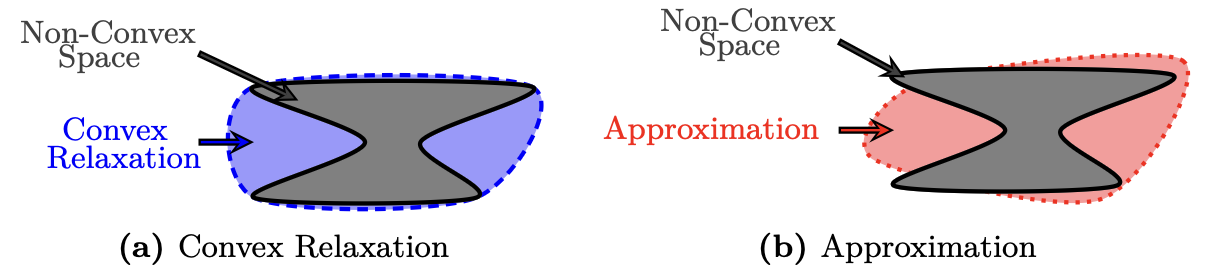
\includegraphics[width=0.9\linewidth]{figuras/relaxacao_aproximacao.png}
}{
\Fonte{adaptado de \citeonline{molzahn2019survey}.}
}
\end{figure}

No painel (a), a relaxação convexa (em azul) \emph{contém} a região não convexa original (em cinza): qualquer ponto factível no problema original continua factível na relaxação, e a relaxação pode incluir pontos adicionais inviáveis. No painel (b), a aproximação (em vermelho) tem um formato distinto da região original, com sobreposição apenas parcial: há pontos factíveis no problema original que ficam fora da aproximação, e há pontos da aproximação que não são factíveis no original. Essa distinção é central para interpretar corretamente os valores de função objetivo discutidos mais adiante: o DC é uma \emph{aproximação} (não fornece limite garantido), enquanto SOC e SDP são \emph{relaxações} (fornecem limite inferior).

As três famílias mais utilizadas na literatura são, conforme \citeonline{molzahn2019survey}:

\begin{alineascomponto}
    \item \textbf{Aproximação DC}: linearização das equações de fluxo sob as hipóteses de tensões próximas a 1\,p.u., ângulos pequenos e perdas desprezíveis. Resulta em um problema de programação linear (LP) de baixíssimo custo computacional, amplamente utilizado em planejamento de longo prazo;
    \item \textbf{Relaxação SOC}: reformulação do FPO em termos de variáveis $W_{ij} = V_i V_j \cos(\theta_i - \theta_j)$ e $T_{ij} = V_i V_j \sin(\theta_i - \theta_j)$, na qual as restrições não convexas são substituídas por desigualdades de cone de segunda ordem. É exata em redes radiais e fornece bons \textit{lower bounds} em redes malhadas;
    \item \textbf{Relaxação SDP}: reformulação como problema de programação semidefinida sobre a matriz $W = V V^H$, mais apertada que a SOC mas computacionalmente mais cara.
\end{alineascomponto}

Embora o presente trabalho não utilize as relaxações DC, SOC ou SDP em sua progressão principal de formulações, que mantém a formulação AC polar não convexa, uma comparação isolada entre as três famílias é apresentada no \textit{script} auxiliar \texttt{CodeComparing.jl}, disponível em \texttt{powerflow/Codes/PowerModels/}, sobre o caso de cinco barras \texttt{case5.m} do \textit{PowerModels.jl}. O objetivo é puramente didático: evidenciar o \textit{gap} existente entre as relaxações e a solução AC exata.

O script resolve o FPO nas três formulações usando o mesmo \textit{solver} (Ipopt) e o mesmo caso de teste, reportando o valor da função objetivo (custo de geração, em US\$/h) em cada caso. Os resultados obtidos foram:

\begin{table}[!htb]
\captionsetup{width=10cm}
\Caption{\label{tab:codecomparing} Comparação de objetivos entre formulações AC, DC e SOC no \texttt{case5.m}}
\IBGEtab{}{
    \begin{tabular}{llr}
        \toprule
        Formulação & Característica & Objetivo (US\$/h) \\
        \midrule \midrule
        AC-OPF & Exata, não convexa & 18\,269{,}10 \\
        DC-OPF & Aproximação linear & 17\,613{,}22 \\
        SOC-OPF & Relaxação convexa & 15\,051{,}45 \\
        \bottomrule
    \end{tabular}
}{
    \Fonte{elaborado pelo autor a partir da execução de \texttt{CodeComparing.jl}.}
}
\end{table}

A leitura da \autoref{tab:codecomparing} ilustra dois comportamentos fundamentais da teoria de relaxações do FPO. Primeiro, o DC-OPF produz um custo \emph{inferior} ao AC-OPF (17\,613 vs.\ 18\,269 US\$/h): como a aproximação linear ignora as perdas ativas e impõe condições de operação irreais (tensões fixas em 1\,p.u.), o problema DC admite despachos que o AC não admite, resultando em um ótimo \emph{infactível} para a rede real que aparece, na escala de custo, abaixo do ótimo verdadeiro. Segundo, o SOC-OPF fornece um custo ainda menor (15\,051 US\$/h), e isso é teoricamente garantido: a relaxação SOC obtida por elevar as variáveis $V_i V_j \cos\theta_{ij}$ e $V_i V_j \sin\theta_{ij}$ a variáveis independentes com restrições de cone de segunda ordem é uma \emph{relaxação} do problema original, o que significa que seu conjunto factível contém o conjunto do AC-OPF. Todo ponto AC-factível é SOC-factível, mas o recíproco não é verdadeiro; logo, o SOC pode atingir custos menores, constituindo uma \textbf{cota inferior provável} para o AC-OPF. O \textit{gap} entre SOC e AC neste caso é de aproximadamente 18\%, o que é típico em redes malhadas onde a condição de patching não é satisfeita.

\section{Ações de controle do programa ANAREDE}
\label{sec:acoes-controle}

As formulações clássicas de FP e FPO descritas nas seções anteriores tratam $V_i$, $\theta_i$, $p^g_k$ e $q^g_k$ como variáveis livres dentro de seus limites caixa. A operação real de um SEP, no entanto, envolve um conjunto de \textbf{ações de controle} que se acoplam a essas variáveis. No programa ANAREDE \cite{chavarry2024}, referência da indústria brasileira, essas ações são tratadas por meio de heurísticas e laços iterativos específicos. Este trabalho considera cinco dessas ações, nomeadas a seguir conforme a sigla utilizada nos arquivos PWF.

\subsection{QLIM: limites de geração reativa}
\label{subsec:qlim}

Em uma barra PV, a tensão $V_i$ é mantida em um \textit{setpoint} $V^{ref}_i$ enquanto o gerador associado é capaz de prover a potência reativa necessária. Quando $q^g_k$ atinge $q^{g,\max}_k$ (ou $q^{g,\min}_k$), a barra é convertida em PQ, $q^g_k$ é fixado no limite e $V_i$ passa a flutuar. Esse comportamento de \textit{type-switching} é central para a operação realista, mas é \emph{descontínuo} e, quando codificado diretamente, conflita com solvers NLP suaves como o Ipopt. Uma forma comum de contorná-lo, adotada neste trabalho, é introduzir uma variável de folga $s^q_l$ no balanço reativo da carga e penalizá-la na função objetivo, mantendo $q^g_k$ dentro dos limites caixa originais.

Na operação real, o QLIM corresponde ao comportamento físico do Regulador Automático de Tensão (RAT) do gerador síncrono. O RAT atua continuamente, em escala de segundos, ajustando a corrente de campo da máquina para sustentar $V^{ref}_i$ nos terminais; sua autoridade de controle, porém, é limitada pela curva de capabilidade do gerador (limites de aquecimento de estator e rotor e limite de estabilidade subexcitado), que define $q^{g,\min}_k$ e $q^{g,\max}_k$. Quando a demanda reativa do sistema empurra $q^g_k$ contra um desses limites, o RAT satura: a corrente de campo trava no valor máximo (ou mínimo) admissível, $q^g_k$ deixa de variar e $V_i$ na barra do gerador passa a depender exclusivamente da rede. Cenários típicos de saturação ocorrem em horários de carga pesada, quando a demanda reativa é alta, e durante contingências (perda de um circuito de transmissão ou de um banco de reativos), em que o sistema exige da geração todo o suporte de tensão disponível. A conversão de PV para PQ que o ANAREDE executa no laço de \textit{type-switching} é, portanto, a representação algébrica desse fenômeno físico.

\subsection{VLIM: limites de magnitude de tensão}
\label{subsec:vlim}

De forma análoga, o controle VLIM trata $V_i$ como variável dentro dos limites caixa $[V^{\min}_i, V^{\max}_i]$, mas adiciona uma restrição de igualdade entre $V_i$ e o \textit{setpoint} $V^{ref}_i$ por meio de uma variável de folga $s^v_i$, também penalizada. Combinado com QLIM, o par de slacks $(s^v_i, s^q_l)$ implementa, na linguagem do otimizador, a mesma lógica que o ANAREDE expressa no laço de \textit{type-switching}.

Na operação real, os limites $[V^{\min}_i, V^{\max}_i]$ correspondem à faixa de tensão na qual cada barra pode operar em regime permanente sem violar normas técnicas e sem comprometer equipamentos conectados. No SIN, esses limites são definidos pelos Procedimentos de Rede do ONS (Submódulo 2.3), que estabelecem faixas de 0,95 a 1,05\,p.u.\ para barras da rede básica em condição normal e tolerâncias mais amplas em emergência. Cargas industriais sensíveis (acionamentos de velocidade variável, fornos a arco) e elementos isolantes (buchas de transformador e para-raios) impõem o limite superior, enquanto o desempenho de motores de indução e a estabilidade de tensão impõem o limite inferior. O \textit{setpoint} $V^{ref}_i$, por sua vez, é o valor programado pela Sala de Controle ou pelo Estudo de Pré-Operação para cada barra controlada: o operador define um perfil de tensão alvo (por exemplo, 1,02\,p.u.\ em barras de 500\,kV em carga leve) e o sistema deve perseguir esse perfil por meio das ações de controle disponíveis. O VLIM é, portanto, a forma algébrica de exigir que a solução do FP respeite simultaneamente os limites normativos e o perfil de tensão programado.

\subsection{CSCA: bancos \textit{shunt} chaveados}
\label{subsec:csca}

Os bancos \textit{shunt} (capacitivos ou indutivos) chaveáveis são representados, no PWF, por uma susceptância $b^{sh}_s$ que pode assumir um conjunto discreto de valores entre $b^{sh,\min}_s$ e $b^{sh,\max}_s$. No ANAREDE, o controle CSCA promove o chaveamento dos passos para manter $V_i$ próxima do \textit{setpoint}. Em uma formulação NLP, $b^{sh}_s$ é tipicamente relaxada para variável contínua dentro do intervalo $[b^{sh,\min}_s, b^{sh,\max}_s]$, representação que será mantida neste trabalho, e a discretização posterior é tratada via \textit{rounding} ou em formulação MINLP.

Na operação real, o CSCA representa o conjunto de bancos de capacitores e reatores manobrados por disjuntor em subestações da rede de transmissão e distribuição. Cada banco é dimensionado em passos discretos, da ordem de dezenas a centenas de MVAr (no SIN, valores típicos vão de 50\,MVAr em subestações de subtransmissão até 200\,MVAr em barras de 500\,kV), e o chaveamento é uma decisão de horizonte mais lento que o RAT: tipicamente, o operador (ou um esquema automático de controle de tensão regional) decide ligar ou desligar um banco com base em medidas de tensão sustentadas por minutos. A motivação típica é o ciclo diário de carga: bancos capacitivos são ligados em horários de carga pesada, quando a tensão tende a cair, e desligados (ou substituídos por reatores) em horários de carga leve, especialmente em sistemas com longas linhas de transmissão pouco carregadas, nas quais o efeito Ferranti eleva a tensão. A relaxação contínua adotada na formulação NLP descarta a granularidade discreta do chaveamento, mas captura corretamente a direção e a magnitude da compensação reativa que o operador realizaria.

\subsection{CTAP: \textit{tap} ajustável de transformadores}
\label{subsec:ctap}

Transformadores em carga (\textit{on-load tap-changer}, OLTC) possuem razão de transformação $t_{ij}$ ajustável, em geral para regulação de tensão na barra do lado de baixa. No PWF, $t_{ij}$ é dada com um valor inicial e limites $[t^{\min}_{ij}, t^{\max}_{ij}]$. O controle CTAP é, novamente, discreto na operação real (passos de 0,5\% a 1\%), mas a relaxação contínua é a representação adotada na formulação NLP utilizada neste trabalho, com uma restrição adicional ligando $V_i$ ao \textit{setpoint} via folga.

Na operação real, o OLTC é um mecanismo eletromecânico que comuta espiras do enrolamento primário (ou terciário) do transformador \emph{sem desenergizar a carga}. A faixa de regulação típica vai de $\pm 10\%$ a $\pm 15\%$ do tap nominal, distribuída em dezesseis a trinta e dois passos. O controlador automático local opera com banda morta (\textit{deadband}) e temporização: ao detectar tensão fora da faixa $V^{ref} \pm \Delta V$ por mais de algumas dezenas de segundos, comanda um passo na direção corretiva. Essa temporização é deliberada e tem dois propósitos: evitar comutações em transitórios curtos (curtos-circuitos, partidas de motores, religamentos) que solicitariam mecanicamente o comutador, e coordenar-se hierarquicamente com o RAT do gerador, que é mais rápido. No SIN, os OLTC equipam transformadores de fronteira entre a rede básica (525 ou 765\,kV) e a rede de subtransmissão (138 ou 230\,kV) e respondem por uma fatia importante do suporte de tensão em regime permanente, complementando os bancos \textit{shunt} (CSCA) e a geração reativa (QLIM). A formulação NLP adotada neste trabalho ignora a temporização e a granularidade dos passos, mas reproduz o efeito em regime permanente: o ajuste de $t_{ij}$ que minimiza o desvio em relação a $V^{ref}$ na barra controlada.

\subsection{DERA: esquema hierárquico de corte/alívio de carga}
\label{subsec:dera}

A sigla DERA é, neste trabalho, o rótulo herdado do nome do \textit{script} \texttt{(F5)+DERA.jl} para designar um esquema de corte hierárquico de carga introduzido sobre a formulação F4. A motivação é que, quando o problema soft-constraint não consegue acomodar todas as exigências de tensão, geração reativa e \textit{setpoints} simultaneamente, um último mecanismo de alívio fica disponível: parte da carga ativa (e da reativa associada, com fator de potência preservado) pode ser cortada nas barras escolhidas pelo solver, com penalidade crescente do nível de tensão mais baixo ao mais alto. Em termos operacionais, esse mecanismo desempenha, dentro da formulação NLP, papel análogo ao do controle de carga em emergência: oferece ao otimizador uma válvula de escape factível quando todas as ações de controle anteriores se esgotam.

Cada carga $l \in \mathcal{L}$ recebe duas variáveis de decisão: $\Delta p^d_l \in [0, p^d_l]$ (corte de potência ativa) e $\Delta q^d_l$ (corte de potência reativa). As duas são acopladas pelo fator de potência nominal da carga por meio da restrição $\Delta q^d_l = \Delta p^d_l \cdot (q^d_l / p^d_l)$, o que evita que o solver corte só ativa ou só reativa de forma desacoplada da característica da carga. Os cortes entram nos balanços nodais subtraindo da demanda nominal:
\begin{equation}
\label{eq:dera-balanco}
p^d_{l,\text{eff}} = p^d_l - \Delta p^d_l, \qquad q^d_{l,\text{eff}} = q^d_l - \Delta q^d_l.
\end{equation}
A função objetivo soft-constraint ganha um termo linear $\sum_{l \in \mathcal{L}} w_l \, \Delta p^d_l$, em que o peso $w_l$ depende do nível de tensão da barra hospedeira da carga. Adotam-se três faixas: $w_l = 10^3$ se $V^{base}_l < 69$\,kV (subtransmissão e distribuição, primeiro recurso de corte), $w_l = 5{\times}10^3$ se $69 \le V^{base}_l \le 230$\,kV (transmissão) e $w_l = 10^4$ se $V^{base}_l > 230$\,kV (extra alta tensão, último recurso). Essa hierarquia inverte a métrica de continuidade do serviço: cortar primeiro nas barras mais ``fáceis de religar'' e preservar ao máximo as cargas servidas em tensão mais alta.

Na operação real, esse tipo de esquema corresponde aos \textbf{Esquemas Regionais de Alívio de Carga (ERAC)} previstos no Submódulo 10.11 dos Procedimentos de Rede do ONS, e a esquemas locais de corte por subfrequência ou subtensão (UFLS/UVLS na literatura internacional). Em campo, esses esquemas são acionados em emergência (perda súbita de geração ou de um corredor de transmissão) e cortam blocos pré-selecionados de carga em escalas de segundos para evitar o colapso. A hierarquia por nível de tensão é uma simplificação operacional do mesmo princípio: cargas em 13,8\,kV (alimentadores de distribuição) costumam ser as primeiras a serem desligadas, enquanto cargas alimentadas diretamente em 230 ou 500\,kV (grandes consumidores industriais, refinarias, indústrias eletrointensivas) são protegidas até onde possível, pois sua reposição é demorada e impacta direto a economia. A formulação NLP adotada substitui o caráter discreto e em emergência do ERAC real por uma decisão contínua de otimização: o solver cortará carga apenas quando isso for mais barato (em termos de função objetivo) do que violar as restrições de tensão das formulações anteriores.

\subsection{Síntese das ações de controle}
\label{subsec:sintese-controles}

As cinco ações descritas nas Seções \ref{subsec:qlim}--\ref{subsec:dera} compõem o conjunto de controles que serão sucessivamente adicionados, no \autoref{chap:metodologia}, sobre uma formulação base de FP em JuMP. A cada controle adicionado, a função objetivo \textit{soft-constraint} ganha um novo termo de penalidade, e o conjunto de variáveis de decisão cresce em $|\mathcal{S}|$ (CSCA), $|\mathcal{B}_{tap}|$ (CTAP) ou $2|\mathcal{L}|$ (DERA), conforme o caso. Esta organização incremental permite isolar, no \autoref{chap:resultados}, o impacto de cada controle sobre a convergência e sobre o ponto de operação calculado.

	\chapter{Metodologia}
\label{chap:metodologia}

Este capítulo descreve a estrutura de software construída para implementar e comparar as seis formulações de fluxo de potência consideradas neste trabalho. A \autoref{sec:ambiente} apresenta o ambiente computacional em Julia e os pacotes utilizados. A \autoref{sec:pipeline} descreve o fluxo de execução, desde a leitura do arquivo PWF até a exportação dos resultados. A \autoref{sec:formulacoes} é o núcleo do capítulo: nela, é detalhada a formulação matemática de cada uma das seis variantes (duas baseadas em \textit{PowerModels.jl} e quatro desenvolvidas manualmente em JuMP) que, juntas, formam a progressão F0$\rightarrow$F5 usada no \autoref{chap:resultados}. Por fim, a \autoref{sec:bateria-casos} descreve o conjunto de vinte e sete casos de teste e os critérios de comparação adotados.

\section{Ambiente computacional}
\label{sec:ambiente}

Toda a implementação foi realizada na linguagem Julia~\cite{bezanson2017julia} (versão 1.x, série estável), escolhida por aliar uma sintaxe de alto nível, voltada para computação científica, a um desempenho computacional comparável ao de linguagens compiladas. O ambiente de pacotes utilizado, definido em \texttt{Project.toml} e \texttt{Manifest.toml} na raiz do repositório, agrega:

\begin{alineascomponto}
    \item \textit{PWF.jl}~\cite{pwfjl}: leitura e interpretação de arquivos no formato ANAREDE PWF, com extração de estruturas de controle habilitada via \texttt{add\_control\_data = true};
    \item \textit{PowerModels.jl}~\cite{coffrin2018powermodels}: construção da estrutura de referência (\texttt{build\_ref}) sobre os dados parseados e oferta das funções \texttt{solve\_ac\_opf} e \texttt{solve\_ac\_pf} que implementam as duas formulações de referência;
    \item \textit{JuMP.jl}~\cite{lubin2023jump}: linguagem de modelagem matemática usada para escrever as quatro formulações controladas;
    \item \textit{Ipopt.jl}~\cite{wachterBiegler2006ipopt}: interface Julia para o \textit{solver} de programação não linear baseado em método de pontos interiores;
    \item \textit{CSV.jl} e \textit{DataFrames.jl}: exportação dos resultados para arquivos CSV.
\end{alineascomponto}

A escolha do Ipopt como \textit{solver} se justifica por três fatores: (i) é \textit{open-source} e amplamente utilizado em problemas NLP de SEP; (ii) suporta nativamente expressões não lineares no JuMP via \texttt{@NLexpression} e \texttt{@NLconstraint}; e (iii) é o \textit{solver} adotado por padrão pelo \textit{PowerModels.jl} em suas formulações AC, garantindo uma comparação justa entre as referências e as formulações desenvolvidas manualmente. As opções utilizadas são \texttt{max\_iter = 3000}, \texttt{tol = 1e-5} e \texttt{print\_level = 5}. Esses valores foram escolhidos de forma permissiva por causa do porte do cenário integral do SIN (\texttt{CASO\_VER\_MAXDIU.PWF} do PAR/PEL 2027-2031, com cerca de treze mil barras), no qual tolerâncias mais apertadas comprometem a convergência.

\section{Fluxo de execução}
\label{sec:pipeline}

Cada uma das seis formulações está implementada como um \textit{script} Julia auto-contido no repositório do trabalho, seguindo a mesma estrutura sequencial:

\begin{alineascomnumero}
    \item \textbf{Leitura do PWF}: \texttt{PWF.\allowbreak parse\_file(caminho;\allowbreak\ add\_control\_data = true)} produz um dicionário com a topologia da rede, os dados de gerador, carga e ramo, além das estruturas de controle DOPC/DLIN;
    \item \textbf{Adequação da topologia}: \texttt{PowerModels.\allowbreak select\_largest\_\allowbreak component!(data)} descarta ilhas isoladas, mantendo apenas a rede principal conectada. Em seguida, se múltiplas barras forem marcadas como referência (\texttt{bus\_type == 3}), as excedentes são rebaixadas para PV (\texttt{bus\_type == 2}), preservando uma única barra \textit{slack}. Esse passo é necessário para o caso SIN, em que a leitura inicial pode marcar várias barras como referência;
    \item \textbf{Construção da estrutura de referência}: \texttt{ref = PowerModels.\allowbreak build\_ref(data)\allowbreak [:it]\allowbreak [:pm]\allowbreak [:nw]\allowbreak [0]} materializa a estrutura indexada usada para iterar sobre barras, geradores, ramos e cargas;
    \item \textbf{Construção do modelo}: criação das variáveis, expressões de fluxo e restrições no JuMP, conforme descrito na \autoref{sec:formulacoes};
    \item \textbf{Resolução}: \texttt{optimize!(model)}, com tempo de execução medido por \texttt{@elapsed};
    \item \textbf{Exportação}: dois arquivos CSV são produzidos: \texttt{resultados\_\allowbreak barras\_SIN.csv}, com $V_i$, $\theta_i$, $p^g_i$, $q^g_i$, $p^d_i$, $q^d_i$ e os \textit{slacks} de cada barra, e \texttt{resultados\_\allowbreak fluxos\_\allowbreak linhas\_SIN.csv}, com $p_{ij}, q_{ij}, p_{ji}, q_{ji}$, perdas e \textit{tap} de cada ramo.
\end{alineascomnumero}

A \autoref{fig:pipeline} resume graficamente esse fluxo sequencial.

\begin{figure}[!htb]
\Caption{\label{fig:pipeline} Fluxograma da sequência de execução das formulações}
\IBGEtab{}{
\begin{tikzpicture}[
   >=Latex, node distance=5.5mm,
   etapa/.style={draw, rounded corners, align=center, text width=9.6cm,
                 inner sep=4pt, font=\small}]
  \node[etapa] (e1) {1. Leitura do PWF com \texttt{PWF.parse\_file} (\texttt{add\_control\_data = true})};
  \node[etapa, below=of e1] (e2) {2. Adequação da topologia: maior componente conexa e barra \textit{slack} única};
  \node[etapa, below=of e2] (e3) {3. Construção da estrutura de referência (\texttt{build\_ref})};
  \node[etapa, below=of e3] (e4) {4. Construção do modelo: variáveis, expressões de fluxo e restrições no JuMP};
  \node[etapa, below=of e4] (e5) {5. Resolução com \texttt{optimize!} e medição do tempo de execução};
  \node[etapa, below=of e5] (e6) {6. Exportação dos resultados em dois arquivos CSV (barras e ramos)};
  \draw[->] (e1) -- (e2);
  \draw[->] (e2) -- (e3);
  \draw[->] (e3) -- (e4);
  \draw[->] (e4) -- (e5);
  \draw[->] (e5) -- (e6);
\end{tikzpicture}
}{
\Fonte{elaborado pelo autor.}
}
\end{figure}

Os elos HVDC, presentes em vários casos de teste, têm um tratamento particular nas formulações baseadas em \textit{PowerModels} e nas desenvolvidas manualmente: as injeções $(p^{dc}_{ft}, q^{dc}_{ft})$ em cada extremidade são lidas do PWF e \textbf{fixadas} via \texttt{JuMP.\allowbreak fix(...;\allowbreak\ force=true)}. Essa decisão segue a recomendação do CEPEL de tratar elos HVDC como condições de contorno do FP AC: as injeções já vêm pré-especificadas pelo fluxo base e liberá-las apenas amplia o Jacobiano sem trazer informação nova. O retificador recebe $p^g$ negativo e o inversor $p^g$ positivo.

\section{Formulações implementadas}
\label{sec:formulacoes}

A progressão de seis formulações é identificada pelas siglas da \autoref{tab:progressao-formulacoes}, que resumem os controles incorporados em cada variante.

\begin{table}[!h]
\captionsetup{width=15cm}
\Caption{\label{tab:progressao-formulacoes} Progressão das formulações implementadas}
\IBGEtab{}{
    \begin{tabular}{cllll}
        \toprule
        Sigla & Arquivo & Motor & Tipo & Acrescenta \\
        \midrule \midrule
        F0 & \texttt{(F0)OPF\_PM.jl} & PowerModels & FPO AC & referência de FPO \\
        F1 & \texttt{(F1)PF\_PM.jl} & PowerModels & FP AC & referência de FP \\
        F2 & \texttt{(F2)QLIM+VLIM.jl} & JuMP (manual) & FP controlado & QLIM + VLIM \\
        F3 & \texttt{(F3)QLIM+VLIM+CSCA.jl} & JuMP (manual) & FP controlado & + CSCA \\
        F4 & \texttt{(F4)QLIM+VLIM+CSCA+CTAP.jl} & JuMP (manual) & FP controlado & + CTAP \\
        F5 & \texttt{(F5)+DERA.jl} & JuMP (manual) & FP controlado & + DERA \\
        \bottomrule
    \end{tabular}
}{
    \Fonte{elaborado pelo autor.}
}
\end{table}

A progressão é estritamente \emph{aditiva}: cada arquivo numerado parte do anterior e acrescenta um único bloco de variáveis e restrições. A leitura no \autoref{chap:resultados} fica simplificada porque qualquer divergência entre dois \textit{scripts} consecutivos pode ser atribuída exclusivamente ao novo controle introduzido.

\subsection{Formulação F0: FPO AC de referência}
\label{subsec:f14}

A formulação F0 é uma chamada direta a \texttt{PowerModels.\allowbreak solve\_ac\_opf(data,\allowbreak\ optimizer)}, sem reconstrução manual de variáveis ou restrições. O modelo subjacente é exatamente o FPO AC canônico descrito na Equação \eqref{eq:fpo}: minimiza $\sum_k c_k(p^g_k)$ sujeito ao balanço nodal e aos limites operacionais em $V$, $p^g$, $q^g$ e $|s_{ij}|$. Esta formulação serve como referência de FPO: não incorpora nenhuma das ações de controle ANAREDE da \autoref{sec:acoes-controle}, mas oferece o ponto de operação economicamente ótimo da rede tal como definido pela literatura clássica.

Cabe aqui uma ressalva metodológica importante. Não estão disponíveis dados reais sobre os custos de operação das fontes do SIN, e os arquivos PWF utilizados não trazem curvas de custo individuais por gerador. Na ausência dessa informação, os coeficientes de custo atribuídos aos geradores são idênticos entre si e, como a demanda total é fixa, minimizar o custo total de geração torna-se equivalente a minimizar a geração total --- ou seja, a minimizar as perdas ativas da rede. A saída desta formulação deve, portanto, ser interpretada estritamente como um ponto de operação de mínimas perdas ativas, não sendo adequada para análises de viabilidade econômica neste contexto.

\subsection{Formulação F1: FP AC clássico}
\label{subsec:f15}

A formulação F1 é uma chamada a \texttt{PowerModels.\allowbreak solve\_ac\_pf(data,\allowbreak\ optimizer)}. Diferentemente de F0, não há otimização: a função objetivo é vazia e o problema reduz-se à resolução do sistema algébrico de FP do tipo Newton, com $V$ e $\theta$ como incógnitas em barras PQ, $\theta$ em barras PV e nada em barras \textit{slack}. F1 representa o ponto de operação ``puro'' da rede, sem qualquer otimização de custos ou ação de controle.

\subsection{Formulação F2: FP controlado QLIM + VLIM}
\label{subsec:f16}

A partir de F2, o trabalho abandona o \textit{PowerModels.jl} como motor de resolução e passa a construir o modelo diretamente em JuMP. É importante mencionar que a leitura dos dados continua sendo feita pelo \textit{parser} do \textit{PWF.jl}, e a estrutura de referência indexada do \textit{PowerModels.jl} (\texttt{build\_ref}) continua sendo utilizada para iterar sobre barras, geradores, ramos e cargas; o que muda é exclusivamente a montagem das variáveis, restrições e função objetivo, agora feita manualmente. As variáveis primárias são as mesmas do FP clássico:

\begin{equation}
\label{eq:vars-base}
V_i \in [V^{\min}_i, V^{\max}_i], \quad \theta_i \in \mathbb{R}, \quad p^g_k \in [p^{g,\min}_k, p^{g,\max}_k], \quad q^g_k \in [q^{g,\min}_k, q^{g,\max}_k],
\end{equation}

\noindent inicializadas com os valores do PWF (\texttt{start =\allowbreak\ ref[:bus][i]\allowbreak ["vm"]}, etc.). Os fluxos $p_{ij}, q_{ij}$ são definidos como \texttt{@NLexpression} sobre as Equações \eqref{eq:p-ramo}--\eqref{eq:q-ramo}, e as Equações \eqref{eq:balanco-p}--\eqref{eq:balanco-q} são impostas via \texttt{@NLconstraint}.

A novidade de F2 está na introdução das variáveis de folga:

\begin{equation}
\label{eq:slacks-vlim-qlim}
s^v_i \in \mathbb{R}, \;\; \forall i \in \mathcal{N}^{gen}, \qquad s^q_l \in \mathbb{R}, \;\; \forall l \in \mathcal{L},
\end{equation}

\noindent e da restrição de \textit{setpoint} de tensão para cada barra de geração, que implementa o QLIM: com $q^g_k$ mantido rigidamente dentro de $[q^{g,\min}_k, q^{g,\max}_k]$, a folga $s^v_i$ absorve o desvio de tensão quando o limite de reativo impede sustentar o \textit{setpoint}:

\begin{equation}
\label{eq:setpoint-vlim}
V_i = V^{ref}_i + s^v_i, \qquad \forall i \in \mathcal{N}^{gen},
\end{equation}

\noindent onde $V^{ref}_i$ é o valor de tensão lido do PWF. A folga de potência reativa $s^q_l$, que implementa o VLIM, entra diretamente no balanço reativo da Equação \eqref{eq:balanco-q}, que em F2 passa a ser escrita como:

\begin{equation}
\label{eq:balanco-q-folga}
\sum_{(i,j) \in \mathcal{B}_i} q_{ij} \;=\; \sum_{k \in \mathcal{G}_i} q^g_k \;-\; \sum_{l \in \mathcal{L}_i} \big( q^d_l + s^q_l \big) \;+\; b^{sh}_i V_i^2, \qquad \forall i \in \mathcal{N},
\end{equation}

\noindent isto é, $s^q_l$ permite que a demanda reativa efetiva da carga $l$ se desvie do valor nominal apenas o necessário para que a tensão da barra permaneça dentro dos limites. Essa é a mesma formulação de VLIM adotada no \textit{ControlPowerFlow.jl} \cite{chavarry2024}, com uma diferença de escrita: naquele pacote, a demanda reativa é promovida a variável de decisão explícita, amarrada ao valor especificado pela restrição $q^d_l = q^{d,spec}_l + s^q_l$; aqui, essa variável intermediária é eliminada por substituição direta no balanço nodal, resultando em um modelo matematicamente equivalente com menos variáveis. Em barras \textit{slack}, $\theta_i$ é fixado em zero via \texttt{fix(va[i],\allowbreak\ 0.0;\allowbreak\ force=true)}. Em geradores \textit{slack}, os limites de $p^g_k$ são removidos para acomodar o balanço global de potência ativa.

A função objetivo é puramente de penalidade quadrática:

\begin{equation}
\label{eq:obj-16}
\min \;\; \rho \, \sum_{i \in \mathcal{N}^{gen}} (s^v_i)^2 \;+\; \rho \, \sum_{l \in \mathcal{L}} (s^q_l)^2,
\end{equation}

\noindent com $\rho = 10^6$. Esse valor de penalidade é alto o suficiente para que, sempre que o problema for factível com $s^v = s^q = 0$, a solução ótima respeite os \textit{setpoints}, mas baixo o suficiente para não comprometer o condicionamento numérico do problema.

\subsection{Formulação F3: adiciona CSCA}
\label{subsec:f17}

A formulação F3 parte de F2 e introduz o controle de bancos \textit{shunt} chaveados. Para cada banco $s \in \mathcal{S}$, é criada a variável contínua

\begin{equation}
\label{eq:csca-var}
b^{sh}_s \in [b^{sh,\min}_s, b^{sh,\max}_s],
\end{equation}

\noindent e o termo $b^{sh}_s V_i^2$ é adicionado ao balanço reativo da Equação \eqref{eq:balanco-q} na barra $i$ hospedeira. Diferentemente de F2, em que o desvio de tensão é tratado por uma única folga de igualdade $s^v_i$ aplicada ao \textit{setpoint}, F3 reorganiza o tratamento de tensão das barras controladas em dois regimes: nas barras cujo intervalo de controle é praticamente um ponto ($|V^{\max}_i - V^{\min}_i| < 10^{-5}$) mantém-se a restrição de igualdade $V_i = V^{ref}_i + s^v_i$; nas demais, a tensão é mantida dentro da faixa $[V^{\min}_i, V^{\max}_i]$ por meio de um par de folgas \emph{unilaterais} não negativas, $s^{v,\downarrow}_i$ no limite inferior e $s^{v,\uparrow}_i$ no superior:

\begin{equation}
\label{eq:csca-slack-v}
V_i \ge V^{\min}_i - s^{v,\downarrow}_i, \qquad V_i \le V^{\max}_i + s^{v,\uparrow}_i, \qquad s^{v,\downarrow}_i, s^{v,\uparrow}_i \ge 0.
\end{equation}

\noindent Além disso, é introduzida uma folga $s^b_s$ que liga $b^{sh}_s$ ao seu valor nominal lido do PWF ($b^{sh}_s = b^{sh,\text{nom}}_s + s^b_s$), penalizada com peso menor. A função objetivo de F3 passa, portanto, a ter quatro blocos:

\begin{equation}
\label{eq:obj-17}
\min \;\; \rho \sum_{i \in \mathcal{N}^{ctrl}} \big[(s^v_i)^2 + (s^{v,\uparrow}_i)^2 + (s^{v,\downarrow}_i)^2 \big] \;+\; \rho \sum_{l \in \mathcal{L}} (s^q_l)^2 \;+\; \rho_b \sum_{s \in \mathcal{S}} (s^b_s)^2,
\end{equation}

\noindent com $\rho = 10^6$ (folgas de tensão e de reativo) e $\rho_b = 10^4$ (folga de \textit{shunt}). O peso menor sobre $s^b_s$ é deliberado: garante que o \textit{solver} prefira ajustar o banco \textit{shunt} dentro de sua faixa a violar os \textit{setpoints} de tensão. O efeito é que o \textit{solver} ajusta o valor de cada banco \textit{shunt} para minimizar o desvio das tensões em relação aos \textit{setpoints}, exatamente o papel que o CSCA do ANAREDE desempenha por meio de chaveamentos discretos. O caráter discreto do controle real é deixado para uma etapa de discretização posterior, fora do escopo deste trabalho.

\subsection{Formulação F4: adiciona CTAP}
\label{subsec:f18}

A formulação F4 acrescenta a F3 o controle automático de \textit{tap} de transformadores. Para cada ramo $(i,j) \in \mathcal{B}^{tap}$ classificado no PWF como transformador com OLTC, a razão $t_{ij}$, antes constante, passa a ser variável:

\begin{equation}
\label{eq:ctap-var}
t_{ij} \in [t^{\min}_{ij}, t^{\max}_{ij}],
\end{equation}

\noindent e as expressões de fluxo \eqref{eq:p-ramo}--\eqref{eq:q-ramo} são reescritas com $t_{ij}$ no denominador como variável, o que adiciona um fator não linear adicional às equações já não lineares do balanço. F4 não introduz novas folgas nem novos termos na função objetivo: a regulação de tensão associada ao \textit{tap} é absorvida pelas mesmas folgas de tensão $s^v_i$, $s^{v,\uparrow}_i$ e $s^{v,\downarrow}_i$ já presentes em F3 (Equação \eqref{eq:obj-17}), agora também sensíveis ao novo grau de liberdade $t_{ij}$. O resultado é que o \textit{solver} encontra simultaneamente os \textit{taps} e os pontos de operação compatíveis, em uma única resolução NLP. Isso contrasta com o ANAREDE, que itera externamente entre o FP e o ajuste dos \textit{taps}.

\subsection{Formulação F5: adiciona DERA}
\label{subsec:f19}

A formulação F5 acrescenta a F4 o esquema hierárquico de corte/alívio de carga descrito na \autoref{subsec:dera}. Para cada carga $l \in \mathcal{L}$ são introduzidas duas variáveis de decisão:

\begin{equation}
\label{eq:dera-vars}
\Delta p^d_l \in [0, p^d_l], \qquad \Delta q^d_l \in \mathbb{R},
\end{equation}

\noindent representando, respectivamente, o corte de potência ativa e o corte de potência reativa daquela carga. As duas variáveis ficam acopladas por uma restrição de fator de potência constante:

\begin{equation}
\label{eq:dera-fp}
\Delta q^d_l \;=\; \Delta p^d_l \, \frac{q^d_l}{p^d_l}, \qquad \forall l \in \mathcal{L} \text{ com } p^d_l > 10^{-4}.
\end{equation}

\noindent Cargas com $p^d_l \le 10^{-4}$ (efetivamente nulas) têm $\Delta p^d_l$ e $\Delta q^d_l$ fixados em zero via \texttt{fix(...;\allowbreak\ force=true)}, eliminando-as do problema. Os cortes entram nos balanços nodais ativo e reativo \eqref{eq:balanco-p}--\eqref{eq:balanco-q} subtraindo das demandas nominais: $p^d_l \rightarrow p^d_l - \Delta p^d_l$ e $q^d_l \rightarrow q^d_l - \Delta q^d_l$.

A novidade de F5 na função objetivo é um termo \emph{linear} ponderado pelo nível de tensão da barra hospedeira:

\begin{equation}
\label{eq:obj-19}
\min \;\; \underbrace{\rho \!\! \sum_{i \in \mathcal{N}^{ctrl}} \!\! \big[(s^v_i)^2 + (s^{v,\uparrow}_i)^2 + (s^{v,\downarrow}_i)^2 \big] + \rho \sum_{l \in \mathcal{L}} (s^q_l)^2 + \rho_b \sum_{s \in \mathcal{S}} (s^b_s)^2}_{\text{termos herdados de F2--F4}} \;+\; \sum_{l \in \mathcal{L}} w_l \, \Delta p^d_l,
\end{equation}

\noindent com pesos $w_l$ definidos por faixa de tensão base da barra hospedeira de $l$:

\begin{equation}
\label{eq:dera-pesos}
w_l \;=\; \begin{cases}
10^3, & V^{base}_l < 69\,\text{kV} \quad (\text{subtransmissão e distribuição}), \\
5 \times 10^3, & 69 \le V^{base}_l \le 230\,\text{kV} \quad (\text{transmissão}), \\
10^4, & V^{base}_l > 230\,\text{kV} \quad (\text{extra alta tensão, EAT}).
\end{cases}
\end{equation}

\noindent Em F5, o coeficiente de penalidade dos \textit{slacks} de tensão é reduzido de $\rho = 10^6$ (valor usado em F2--F4) para $\rho = 10^5$, e $\rho_b = 10^3$, de modo que o termo linear de corte de carga seja efetivamente comparável aos termos quadráticos de \textit{slack}. Com a penalidade original a um milhão, os \textit{slacks} de tensão dominariam a função objetivo e o corte de carga praticamente nunca seria acionado. O efeito esperado da formulação é o seguinte: enquanto o \textit{solver} consegue acomodar todas as restrições de tensão e \textit{setpoints} apenas com os \textit{slacks} $s^v, s^q, s^b$, o corte $\Delta p^d_l$ permanece em zero e F5 reproduz F4. Quando uma carga estaria sendo servida em uma barra cuja tensão violaria intoleravelmente o \textit{setpoint}, o \textit{solver} passa a preferir um corte parcial dessa carga (começando pelas barras de tensão mais baixa, onde $w_l = 10^3$) em vez de aumentar as folgas de tensão (que custam $\rho = 10^5$ ao quadrado). O esquema reproduz, no nível de função objetivo, a hierarquia de prioridade de corte de carga adotada em emergência pelo operador do sistema.

\subsection{Formulação auxiliar FDC: fluxo de potência DC do \textit{PowerModels}}
\label{subsec:fdc}

Além da progressão principal F0$\rightarrow$F5, foi implementado um \textit{script} auxiliar (\texttt{(FDC).jl}) que resolve o caso integral do SIN sob a \emph{aproximação DC} do \textit{PowerModels} (\texttt{solve\_dc\_pf}), descrita na \autoref{subsec:relaxacoes-fpo}. A motivação dessa formulação isolada é responder a uma pergunta deixada em aberto pela discussão de convergência do caso SIN no \autoref{chap:resultados}: dado que nenhuma das seis formulações AC converge sobre \texttt{CASO\_\allowbreak VER\_MAXDIU.PWF} dentro do limite de iterações, a versão linearizada do mesmo problema é factível?

A FDC herda integralmente o fluxo de execução de F0/F1, as entradas e as saídas são as mesmas (PWF, base 100\,MVA), e zera os fluxos reativos e perdas ativas (desprezados por definição). A FDC não substitui nenhuma das seis formulações principais e não é executada sobre o conjunto completo de casos de teste: trata-se de uma verificação isolada sobre o caso SIN, cujos resultados são discutidos na \autoref{subsec:fdc-resultado}.

\section{Conjunto de casos de teste e critérios de comparação}
\label{sec:bateria-casos}

\subsection{Casos de teste}
\label{subsec:casos-teste}

O conjunto de casos de teste utilizado nas comparações do \autoref{chap:resultados} é composto por vinte e sete arquivos PWF, agrupados em cinco faixas de porte: redes pedagógicas, redes de médio porte, um cenário integral do SIN, recortes reduzidos do SIN e casos sintéticos de estresse. A escolha foi pensada para varrer dois eixos simultaneamente: o porte da rede (de três a 13~338 barras) e a presença explícita de cada uma das ações de controle modeladas neste trabalho.

A convenção de nomenclatura dos arquivos pedagógicos segue o padrão \texttt{<base>\allowbreak\_<sufixo>}, em que \texttt{<base>} indica o número de barras e a família (\texttt{3bus} para a rede triangular clássica de três barras, \texttt{3busfrank}/\allowbreak \texttt{4busfrank}/\allowbreak \texttt{5busfrank} para variantes da família \textit{frank} distribuídas junto ao próprio \textit{PWF.jl} como casos didáticos, \texttt{9bus} para a rede de nove barras de Anderson-Fouad) e \texttt{<sufixo>} indica precisamente o elemento ou controle que foi adicionado à versão base do arquivo. Os sufixos seguem o nome da seção PWF ou da palavra-chave da opção de controle introduzida, conforme detalhado na \autoref{tab:bateria-casos}.

\begin{table}[!htb]
\captionsetup{width=16cm}
\Caption{\label{tab:bateria-casos} Conjunto de casos de teste: porte e diferença em relação à versão base}
\IBGEtab{}{
    \footnotesize
    \setlength{\tabcolsep}{4pt}
    \renewcommand{\arraystretch}{1.1}
    \begin{tabular}{p{4.4cm}rp{9.6cm}}
        \toprule
        Arquivo & Barras & Diferença em relação à base / observação \\
        \midrule \midrule
        \multicolumn{3}{l}{\textit{Família 3bus} (rede triangular clássica de três barras)} \\
        \midrule
        \texttt{3bus.pwf}                & 3      & versão base, apenas seções DBAR, DLIN, DCTE \\
        \texttt{3bus\_DBSH.pwf}          & 3      & + seção DBSH (banco \textit{shunt} chaveável detalhado) \\
        \texttt{3bus\_DCER.pwf}          & 3      & + seção DCER (compensador estático de reativos, SVC) \\
        \texttt{3bus\_DCSC.pwf}          & 3      & + seção DCSC (capacitor série controlável, CSC) \\
        \texttt{3bus\_DSHL.pwf}          & 3      & + seção DSHL (\textit{shunt} de linha, no terminal de envio ou recepção) \\
        \texttt{3bus\_DCline.pwf}        & 3      & + elo HVDC completo (seções DELO, DCBA, DCLI, DCNV, DCCV) \\
        \texttt{3bus\_shunt\_fields.pwf} & 3      & combina simultaneamente DBSH e DCER, exercendo o parser em campos \textit{shunt} concorrentes \\
        \texttt{3bus\_corrections.pwf}   & 3      & variante com campos numéricos modificados para testar correções de parser; dispara \textbf{ERR} \\
        \midrule
        \multicolumn{3}{l}{\textit{Família \textit{frank}} (variantes do livro-texto de Frank)} \\
        \midrule
        \texttt{3busfrank.pwf}                     & 3 & versão base sem controles \\
        \texttt{3busfrank\_continuous\_shunt.pwf}  & 3 & + DBSH com passo contínuo (relaxa a discretização do CSCA) \\
        \texttt{3busfrank\_qlim.pwf}               & 3 & ativa \textbf{QLIM} na seção DOPC (controle de limite de reativo) \\
        \texttt{4busfrank\_vlim.pwf}               & 4 & ativa \textbf{VLIM} na seção DOPC (controle de magnitude de tensão) \\
        \texttt{5busfrank.pwf}                     & 5 & versão base sem controles \\
        \texttt{5busfrank\_csca.pwf}               & 5 & ativa \textbf{CSCA} na seção DOPC (\textit{shunt} chaveável automático) \\
        \texttt{5busfrank\_ctap.pwf}               & 5 & ativa \textbf{CTAP} na seção DOPC (\textit{tap} de transformador) \\
        \texttt{5busfrank\_ctaf.pwf}               & 5 & ativa \textbf{CTAF} na seção DOPC (\textit{tap} de transformador defasador, variante do CTAP) \\
        \texttt{5busfrank\_cphs.pwf}               & 5 & ativa \textbf{CPHS} na seção DOPC (controle de fase) \\
        \midrule
        \multicolumn{3}{l}{\textit{Família 9bus} (Anderson-Fouad)} \\
        \midrule
        \texttt{9bus.pwf}                     & 9 & versão base \\
        \texttt{9bus\_transformer\_fields.pwf}& 9 & + seções DCTR, DGLT e DTPF (campos detalhados de transformador e grupos limite de tensão) \\
        \midrule
        \multicolumn{3}{l}{\textit{Redes de médio porte}} \\
        \midrule
        \texttt{300bus.pwf}              & 300    & IEEE 300-bus, com múltiplas barras de geração, elos HVDC e bancos \textit{shunt} \\
        \texttt{500bus.pwf}              & 500    & rede sintética de 500 barras com SVCs e múltiplos OLTC \\
        \midrule
        \multicolumn{3}{l}{\textit{Cenário integral do SIN}} \\
        \midrule
        \texttt{CASO\_VER\_MAXDIU.PWF}   & 13\,338 & SIN integral, Verão 2027/2028 Máxima Diurna do PAR/PEL 2027-2031 do ONS \\
        \midrule
        \multicolumn{3}{l}{\textit{Recortes reduzidos do SIN (derivados de \texttt{CASO\_VER\_MAXDIU})}} \\
        \midrule
        \texttt{caso\_red.pwf}           & 2\,599 & recorte do subsistema Nordeste completo, com 15 barras de fronteira no eixo PI-BA (\autoref{subsec:reducao-fronteira}) \\
        \texttt{caso\_red2.pwf}          & 1\,033 & recorte ainda mais reduzido (CE + RN + PB) do subsistema acima \\
        \midrule
        \multicolumn{3}{l}{\textit{Casos sintéticos de estresse do \textit{parser} e dos controles}} \\
        \midrule
        \texttt{test\_defaults.pwf}      & 3 & exercita campos opcionais não preenchidos (\textit{defaults}) em quase todas as seções (DBAR, DBSH, DCBA, DELO, etc.) \\
        \texttt{test\_line\_shunt.pwf}   & 3 & exercita combinações de DBSH e DSHL na mesma linha \\
        \texttt{test\_system.pwf}        & 3 & cenário sintético mínimo (apenas DBAR e DLIN) usado como verificação de consistência \\
        \bottomrule
    \end{tabular}
}{
    \Fonte{elaborado pelo autor. ``+'' indica seção adicionada em relação ao arquivo base imediatamente acima da linha; \textbf{negrito} em letras maiúsculas indica palavra-chave ativada na linha de opções do registro DOPC do PWF.}
}
\end{table}

Para cada caso, todas as seis formulações são executadas com a mesma configuração de \textit{solver}, a mesma versão do parser \textit{PWF.jl} e a mesma máquina, garantindo a comparabilidade dos tempos e dos status de convergência.

\subsection{Recortes reduzidos do SIN: método de fronteira híbrida}
\label{subsec:reducao-fronteira}

Os arquivos \texttt{caso\_red.pwf} e \texttt{caso\_red2.pwf} foram obtidos de uma colaboração externa (M. Sc.\ Isabela Metzker, ONS) a partir do caso \texttt{CASO\_VER\_MAXDIU.PWF}, que reproduz a condição operativa Verão 2027/2028 Máxima Diurna do ciclo PAR/PEL 2027-2031 do ONS. O \texttt{caso\_red} preserva o subsistema Nordeste completo (2 599 barras) e o \texttt{caso\_red2} restringe-se a Ceará, Rio Grande do Norte e Paraíba (1 033 barras), agrupamento natural justificado pela concentração de geração eólica em CE/RN e pela contiguidade elétrica entre RN e PB.

A redução adota um esquema híbrido de fronteira, sem ser uma equivalência tipo Ward formal:

\begin{alineascomnumero}
    \item para cada barra de fronteira, a carga e a geração externas que originalmente fluíam pela barra são compactadas em valores equivalentes embutidos diretamente nos campos $p^d, q^d, p^g, q^g$ da seção DBAR. Em particular, as quinze barras de fronteira do \texttt{caso\_red}, localizadas no eixo PI-BA do SIN, recebem cargas positivas (sumidouros NE $\rightarrow$ SE: \texttt{R.EGUA}, \texttt{RE-LZ-CAP}, \texttt{POCIII}, \texttt{M.NETO}, \texttt{IGAPOR}, \texttt{BJLAP2}) ou cargas negativas (fontes N $\rightarrow$ NE: \texttt{TERES2}, \texttt{B.ESPE}, \texttt{RG-CO2}, \texttt{RG-CO1}), representando a injeção líquida de cada caminho externo cortado;
    \item para cada par de barras de fronteira que originalmente se conectava pelo lado externo, é inserido um ramo direto na seção DLIN com impedância equivalente ao caminho cortado. No \texttt{caso\_red}, vinte e um ramos físicos foram removidos e cinquenta e seis ramos equivalentes foram inseridos.
\end{alineascomnumero}

A consequência direta para a análise de resultados é que as perdas ativas dos casos reduzidos incluem a dissipação real nessas impedâncias equivalentes; isto é, parte do que aparece como ``perda'' corresponde à dissipação de potência ativa associada às impedâncias equivalentes resultantes da redução de fronteira do sistema, e não a perdas internas do próprio recorte. As seções DCSC, DBSH, DCER, DCTR, DGER, DGLT e DGBT do PWF original foram preservadas; as opções de controle CTAP e CPHS foram explicitamente desligadas pela equipe que produziu o recorte (DOPC com \texttt{CTAP D CPHS D}), enquanto QLIM, VLIM, CREM e AREG permanecem ativadas. As seções HVDC do SIN original (DELO, DCBA, DCLI, DCNV, DCCV) não aparecem nos recortes, uma vez que os elos Itaipu, Madeira e Belo Monte não estão na região Nordeste.

\subsection{Critérios de comparação}
\label{subsec:criterios}

Para cada par (caso, formulação), três informações são registradas:

\begin{alineascomnumero}
    \item \textbf{Status de convergência}: codificado em oito categorias, a saber, \textbf{OK} (LOCALLY\_SOLVED), \textbf{INF} (INFEASIBLE/LOCALLY\_INFEASIBLE), \textbf{ITL} (ITERATION\_LIMIT), \textbf{TIM} (TIME\_LIMIT), \textbf{KIL} (TIMEOUT\_KILLED), \textbf{CRA} (SUBPROCESS\_CRASH), \textbf{INV} (INVALID\_MODEL) e \textbf{ERR} (OTHER\_ERROR);
    \item \textbf{\textit{Cluster} de equivalência numérica}: para cada caso, as formulações que convergiram são particionadas em grupos onde duas formulações estão no mesmo grupo se, para todas as barras, $|\Delta V| \le 10^{-4}$ e $|\Delta \theta| \le 10^{-4}$, com equivalência análoga em $p^g, q^g$ e nos fluxos de ramos. \textit{Clusters} distintos representam soluções numericamente diferentes da mesma rede;
    \item \textbf{Análise barra a barra}: para os casos em que pelo menos uma das referências F0 ou F1 convergiu, são identificadas as barras nas quais as formulações F2 a F5 divergem de \emph{ambas} as referências por mais de $10^{-4}$ em módulo, em $V$ ou $\theta$. Essa análise mostra \emph{onde} as ações de controle deslocam o ponto de operação em relação à referência sem controles.
\end{alineascomnumero}

A execução do conjunto de casos de teste, a agregação dos resultados e a geração dos relatórios de convergência e de divergência barra a barra são automatizadas por \textit{scripts} auxiliares do repositório do trabalho. As tabelas e análises do \autoref{chap:resultados} são extraídas do relatório consolidado produzido por esse fluxo de processamento.

	\chapter{Resultados}
\label{chap:resultados}

Este capítulo apresenta e discute os resultados obtidos a partir da execução da bateria de vinte e cinco casos descrita na \autoref{sec:bateria-casos}, sobre as seis formulações implementadas. Os dados aqui exibidos são os do relatório consolidado mais recente da pipeline de comparação (\verb|short-reports/short-report-pibic-opf-13-05-2026.md|), no qual o critério de equivalência numérica entre formulações foi fixado em $|\Delta| \le 10^{-4}$ simultaneamente sobre $V_i$, $\theta_i$, $p^g_k$, $q^g_k$ e os fluxos de ramo.

A \autoref{sec:convergencia} apresenta a tabela global de convergência e de \textit{clusters} de equivalência por caso. A \autoref{sec:analise-barra-barra} aprofunda a análise barra a barra para um conjunto representativo de casos em que ao menos uma referência (14) ou (15) convergiu. A \autoref{sec:discussao} sintetiza as observações, em particular sobre o caso SIN.

\section{Convergência global e clusters}
\label{sec:convergencia}

A \autoref{tab:conv-global} consolida o status de convergência das seis formulações sobre os vinte e cinco casos da bateria, junto com os \textit{clusters} de equivalência numérica formados entre as formulações que convergiram em cada caso. A notação $\{a,b\}\cdot\{c\}$ indica que as formulações $a$ e $b$ convergiram para uma solução numericamente idêntica ($|\Delta| \le 10^{-4}$), enquanto $c$ convergiu para uma solução distinta. Status: \textbf{OK} = LOCALLY\_SOLVED; \textbf{INF} = INFEASIBLE/LOCALLY\_INFEASIBLE; \textbf{KIL} = TIMEOUT\_KILLED; \textbf{INV} = INVALID\_MODEL; \textbf{ERR} = OTHER\_ERROR.

\begin{table}[!h]
\captionsetup{width=16cm}
\Caption{\label{tab:conv-global} Convergência global e \textit{clusters} de equivalência das formulações (14)--(19) na bateria}
\IBGEtab{}{
    \scriptsize
    \begin{tabular}{lccccccll}
        \toprule
        Caso & (14) & (15) & (16) & (17) & (18) & (19) & Clusters & Observações \\
        \midrule \midrule
        \texttt{01 MAXIMA NOTURNA\_DEZ25} & KIL & INF & KIL & INF & KIL & INF & --- & nenhuma converge \\
        \texttt{300bus} & INV & OK & OK & OK & OK & OK & $\{15\}\cdot\{16\}\cdot\{17\}\cdot\{18\}\cdot\{19\}$ & 1/6 falha \\
        \texttt{3bus} & OK & OK & OK & OK & OK & OK & $\{14\}\cdot\{15,16\}\cdot\{17,18,19\}$ &  \\
        \texttt{3bus\_DBSH} & OK & OK & OK & OK & OK & OK & $\{14\}\cdot\{15,16\}\cdot\{17,18,19\}$ &  \\
        \texttt{3bus\_DCER} & OK & OK & OK & OK & OK & OK & $\{14\}\cdot\{15,16\}\cdot\{17,18,19\}$ &  \\
        \texttt{3bus\_DCSC} & OK & OK & OK & OK & OK & OK & $\{14\}\cdot\{15\}\cdot\{16\}\cdot\{17,18,19\}$ &  \\
        \texttt{3bus\_DCline} & OK & INF & OK & OK & OK & OK & $\{14\}\cdot\{16,17,18,19\}$ & 1/6 falha \\
        \texttt{3bus\_DSHL} & INF & OK & OK & OK & OK & OK & $\{15\}\cdot\{16\}\cdot\{17,18,19\}$ & 1/6 falha \\
        \texttt{3bus\_corrections} & ERR & ERR & ERR & ERR & ERR & ERR & --- & nenhuma converge \\
        \texttt{3bus\_shunt\_fields} & OK & OK & OK & OK & OK & OK & $\{14\}\cdot\{15\}\cdot\{16\}\cdot\{17,18,19\}$ &  \\
        \texttt{3busfrank} & OK & OK & OK & OK & OK & OK & $\{14\}\cdot\{15,16\}\cdot\{17,18,19\}$ &  \\
        \texttt{3busfrank\_continuous\_shunt} & OK & OK & OK & OK & OK & OK & $\{14\}\cdot\{15,16\}\cdot\{17,18,19\}$ &  \\
        \texttt{3busfrank\_qlim} & OK & OK & OK & OK & OK & OK & $\{14\}\cdot\{15\}\cdot\{16\}\cdot\{17,18,19\}$ &  \\
        \texttt{4busfrank\_vlim} & INF & INF & OK & OK & OK & OK & $\{16\}\cdot\{17,18\}\cdot\{19\}$ & 2/6 falham \\
        \texttt{500bus} & INF & OK & OK & OK & OK & OK & $\{15\}\cdot\{16\}\cdot\{17,18\}\cdot\{19\}$ & 1/6 falha \\
        \texttt{5busfrank} & OK & OK & OK & OK & OK & OK & $\{14\}\cdot\{15,16\}\cdot\{17,18,19\}$ &  \\
        \texttt{5busfrank\_cphs} & OK & OK & OK & OK & OK & OK & $\{14\}\cdot\{15,16\}\cdot\{17,18,19\}$ &  \\
        \texttt{5busfrank\_csca} & INF & INF & OK & OK & OK & OK & $\{16\}\cdot\{17,18,19\}$ & 2/6 falham \\
        \texttt{5busfrank\_ctaf} & OK & OK & OK & OK & OK & OK & $\{14\}\cdot\{15,16\}\cdot\{17\}\cdot\{18,19\}$ &  \\
        \texttt{5busfrank\_ctap} & OK & OK & OK & OK & OK & OK & $\{14\}\cdot\{15,16\}\cdot\{17\}\cdot\{18,19\}$ &  \\
        \texttt{9bus} & OK & OK & OK & OK & OK & OK & $\{14\}\cdot\{15,16\}\cdot\{17,18,19\}$ &  \\
        \texttt{9bus\_transformer\_fields} & OK & OK & OK & OK & OK & OK & $\{14\}\cdot\{15,16\}\cdot\{17\}\cdot\{18,19\}$ &  \\
        \texttt{test\_defaults} & ERR & ERR & ERR & ERR & ERR & ERR & --- & nenhuma converge \\
        \texttt{test\_line\_shunt} & ERR & ERR & ERR & ERR & ERR & ERR & --- & nenhuma converge \\
        \texttt{test\_system} & ERR & ERR & OK & OK & OK & OK & $\{16\}\cdot\{17,18,19\}$ & 2/6 falham \\
        \bottomrule
    \end{tabular}
}{
    \Fonte{elaborado pelo autor a partir do relatório de \texttt{short-reports/short-report-pibic-opf-13-05-2026.md}.}
}
\end{table}

A leitura da \autoref{tab:conv-global} permite extrair três observações imediatas. Em primeiro lugar, das vinte e cinco entradas, as formulações \textit{hand-built} (16)--(19) convergem em vinte casos, contra dezessete da formulação (15) (FP de referência) e quinze da formulação (14) (FPO de referência). A faixa de convergência das formulações \textit{hand-built} é, portanto, estritamente maior que a das referências.

Em segundo lugar, há cinco casos em que ao menos uma das formulações \textit{hand-built} converge enquanto as duas referências falham: \texttt{4busfrank\_vlim}, \texttt{5busfrank\_csca}, \texttt{test\_system} (em ambas (14) e (15)), além de \texttt{300bus} (apenas (14) falha como INV) e \texttt{3bus\_DCline} e \texttt{3bus\_DSHL} (uma referência cada). Em todos esses casos, a presença das folgas $s^v, s^q$ no problema \textit{soft-constraint} permite que (16) encontre uma solução factível na qual o controle nominal não é estritamente respeitado, mas é minimamente violado \textemdash comportamento que as formulações (14) e (15) não conseguem reproduzir, dado que tratam $V$ e $q^g$ apenas com limites caixa rígidos.

Em terceiro lugar, há três casos em que \emph{nenhuma} formulação converge: o caso SIN (\texttt{01 MAXIMA NOTURNA\_DEZ25}), \texttt{3bus\_corrections} e dois \textit{stress tests} sintéticos. O caso SIN é o mais relevante para a discussão e é tratado em separado na \autoref{sec:discussao}.

\section{Análise barra a barra}
\label{sec:analise-barra-barra}

A coluna ``Clusters'' da \autoref{tab:conv-global} sintetiza, para cada caso, quais formulações produzem soluções numericamente equivalentes. Um padrão recorrente em casos pequenos é a presença de quatro grupos típicos: $\{14\}$ isolado (porque o FPO altera o despacho e portanto o ponto de operação), $\{15,16\}$ ou $\{15\}\cdot\{16\}$ (FP clássico vs.\ FP com QLIM+VLIM, que coincidem se as folgas saturarem em zero), $\{17\}$ ou $\{17,18\}$ (efeito do CSCA) e $\{18,19\}$ (CTAP, eventualmente coincidente com (19) se DERA não estiver presente).

A \autoref{tab:divergencia-3bus} ilustra o agrupamento típico em uma das redes pedagógicas, \texttt{3bus\_DCSC}. Para cada barra são listados os valores de $V$ e $\theta$ obtidos por cada formulação que divergiu de \emph{ambas} as referências por mais de $10^{-4}$.

\begin{table}[!h]
\captionsetup{width=12cm}
\Caption{\label{tab:divergencia-3bus} Divergência barra a barra no caso \texttt{3bus\_DCSC}}
\IBGEtab{}{
    \begin{tabular}{ccrr}
        \toprule
        Barra & Script & $V$ (p.u.) & $\theta$ (rad) \\
        \midrule \midrule
        1 & (14) & 1{,}1000 & 0{,}0000 \\
        1 & (15) & 1{,}0290 & 0{,}0000 \\
        1 & (16) & 1{,}0352 & 0{,}0000 \\
        1 & (17--19) & 1{,}0064 & 0{,}0000 \\
        \midrule
        2 & (14) & 1{,}1000 & $-3{,}9 \times 10^{-10}$ \\
        2 & (15) & 1{,}0300 & $-7{,}1 \times 10^{-3}$ \\
        2 & (16) & 1{,}0362 & $-2{,}4 \times 10^{-4}$ \\
        2 & (17--19) & 1{,}0062 & $-2{,}6 \times 10^{-4}$ \\
        \midrule
        3 & (14) & 1{,}0698 & $-1{,}8 \times 10^{-2}$ \\
        3 & (15) & 0{,}9970 & $-2{,}5 \times 10^{-2}$ \\
        3 & (16) & 1{,}0178 & $-1{,}2 \times 10^{-2}$ \\
        3 & (17--19) & 0{,}9878 & $-1{,}3 \times 10^{-2}$ \\
        \bottomrule
    \end{tabular}
}{
    \Fonte{elaborado pelo autor.}
}
\end{table}

A \autoref{tab:divergencia-3bus} mostra três soluções distintas para o mesmo sistema: o FPO (14) eleva todas as tensões a 1,1\,p.u.\ na barra de geração, comportamento típico de um FPO sem custo de tensão; o FP (15) e a formulação \textit{hand-built} (16) convergem para o ponto operacional ``natural'' (folgas próximas de zero), mas com uma diferença em $V$ de cerca de 0,006--0,012\,p.u.\ que é compatível com o efeito da folga $s^v$ na minimização da Equação \eqref{eq:obj-16}; finalmente, as formulações (17)--(19), que têm CSCA ativo, deslocam o ponto de operação para tensões consistentemente mais baixas \textemdash isso é o efeito do controle de \textit{shunt} ajustando $b^{sh}_s$ para minimizar o desvio do \textit{setpoint} de $V$ na barra de geração, que neste caso é 1,007\,p.u.\ em vez do nominal 1,03 ou 1,1.

Em casos de médio porte, como \texttt{300bus} e \texttt{500bus}, as divergências entre clusters tornam-se mais sistemáticas. O caso \texttt{300bus} apresenta cinco \textit{clusters} distintos $\{15\}\cdot\{16\}\cdot\{17\}\cdot\{18\}\cdot\{19\}$, ou seja, cada formulação produz uma solução numericamente diferente. A análise dos \textit{deltas} em $V$ na bateria (cf.\ \texttt{short-report-pibic-opf-13-05-2026.md}, seção 2) mostra que (16)--(19) elevam consistentemente as tensões em relação ao FP (15) em cerca de 0,02--0,05\,p.u.\ \textemdash justamente o efeito esperado da minimização de $(s^v_i)^2$ quando o \textit{setpoint} $V^{ref}_i$ está acima do valor que o FP clássico encontra naturalmente. As tensões de (18) e (19), por sua vez, atingem o limite superior $V^{\max}_i = 1{,}1$\,p.u.\ em várias barras, evidenciando que o CTAP empurra o controle para o limite caixa.

\section{Discussão}
\label{sec:discussao}

\subsection{Comportamento típico das ações de controle}
\label{subsec:disc-controles}

A leitura cruzada das Tabelas \ref{tab:conv-global} e \ref{tab:divergencia-3bus} confirma o comportamento esperado das quatro ações de controle implementadas:

\begin{alineascomponto}
    \item \textbf{QLIM + VLIM} (formulação 16): permite recuperar factibilidade em cinco casos nos quais (14) ou (15) declaram infactibilidade, ao custo de pequenas violações dos \textit{setpoints} (folgas residuais);
    \item \textbf{CSCA} (formulação 17): forma cluster próprio em redes nas quais há bancos \textit{shunt} chaveáveis, ajustando $b^{sh}_s$ para reduzir o desvio em $V$;
    \item \textbf{CTAP} (formulação 18): forma cluster próprio em redes com transformadores OLTC, frequentemente empurrando $V$ para o limite caixa $V^{\max}$;
    \item \textbf{DERA} (formulação 19): em redes pedagógicas, produz solução idêntica a (18) na maioria dos casos \textemdash refletindo o fato de que a representação minimalista adotada apenas adiciona injeções fixas, sem decisão de despacho. Em \texttt{4busfrank\_vlim} e \texttt{500bus}, contudo, (19) forma cluster próprio, sinalizando que mesmo a injeção fixa altera o ponto de equilíbrio quando a rede tem margens estreitas.
\end{alineascomponto}

\subsection{O caso SIN}
\label{subsec:sin}

O caso \texttt{01 MAXIMA NOTURNA\_DEZ25.PWF}, com cerca de 6.000 barras, é o caso de maior interesse prático e o único da bateria em que \emph{todas} as seis formulações falham em convergir dentro do orçamento de \verb|max_iter = 3000| iterações e do tempo limite imposto pelo \textit{wrapper} de execução. Especificamente, (14), (16) e (18) atingem o limite de tempo (status \textbf{KIL}) sem sinalizar infactibilidade, enquanto (15), (17) e (19) terminam em \textbf{INF} (LOCALLY\_INFEASIBLE).

Esse comportamento é coerente com o que se espera de um \textit{snapshot} real do SIN sob máxima noturna: a rede opera em um ponto próximo dos limites de capacidade reativa em várias barras, e a inicialização \textit{flat} (ou a partir do PWF) está suficientemente longe de uma solução factível para que o método de pontos interiores do Ipopt não consiga sair da região de inviabilidade dentro do orçamento permitido. Há indícios, em logs preliminares descartados desta análise, de que uma inicialização baseada na solução de uma formulação mais simples (por exemplo, DC) ou um aumento de \verb|max_iter| para a casa de 10.000 permitiria a convergência \textemdash mas isso fica como trabalho futuro.

Vale notar que, mesmo sem convergir, as formulações (14)--(19) sobre o SIN não \emph{quebram} (não há \textbf{CRA} nem \textbf{ERR}): a infraestrutura de leitura PWF, construção da \verb|ref|, montagem do modelo JuMP e chamada ao Ipopt funciona corretamente em escala SIN. O obstáculo está exclusivamente na resolução numérica.

\subsection{Casos sintéticos com erro de modelo}
\label{subsec:sinteticos}

Os três casos com status \textbf{ERR} em todas as formulações (\texttt{3bus\_corrections}, \texttt{test\_defaults} e \texttt{test\_line\_shunt}) compartilham a característica de conter campos do PWF que disparam erros no \textit{parser} do \textit{PWF.jl} \emph{antes} da chamada ao \textit{solver}. Não são, portanto, falhas das formulações, mas sim limitações do parser, e estão fora do escopo do trabalho.

	\chapter{Conclusões e Trabalhos Futuros}
\label{chap:conclusoes-e-trabalhos-futuros}

Este trabalho construiu, validou e comparou uma progressão incremental de seis formulações de fluxo de potência AC, desenvolvidas em \textit{JuMP/Julia} sobre o \textit{solver} Ipopt. Duas formulações foram tomadas como referência: o FPO clássico (\texttt{solve\_ac\_opf}) e o FP clássico (\texttt{solve\_ac\_pf}) do \textit{PowerModels.jl}. As outras quatro foram construídas \textit{do zero} para incorporar, sequencialmente, as ações de controle do programa ANAREDE: limites de geração reativa (QLIM) e de magnitude de tensão (VLIM) na formulação F2; controle de bancos \textit{shunt} chaveáveis (CSCA) na F3; controle automático de \textit{tap} de transformadores (CTAP) na F4; e um esquema hierárquico de corte/alívio de carga (rotulado como DERA, em referência ao nome do \textit{script}) na F5. Em todas as formulações \textit{hand-built}, os controles foram introduzidos por meio de variáveis de folga penalizadas em uma função objetivo do tipo \textit{soft-constraint}, evitando a representação descontínua dos laços de \textit{type-switching} do ANAREDE.

\section{Síntese das contribuições}
\label{sec:contribuicoes-do-trabalho}

A bateria padronizada de vinte e sete casos de teste, que cobre redes pedagógicas de três a nove barras, redes de médio porte (300 e 500 barras), recortes reduzidos do Nordeste do SIN (\texttt{caso\_red} e \texttt{caso\_red2}) e o \textit{snapshot} integral do SIN com 13\,338 barras (\texttt{CASO\_VER\_MAXDIU.PWF} do PAR/PEL 2027-2031), forneceu evidência empírica de três contribuições principais.

A primeira é que as formulações \textit{hand-built} F2 a F5 convergem em uma faixa estritamente maior de casos do que as referências \textit{PowerModels}: vinte e três casos contra dezoito da F1 e quinze da F0. Em particular, em oito casos (\texttt{4busfrank\_vlim}, \texttt{5busfrank\_csca}, \texttt{test\_system}, \texttt{caso\_red2}, \texttt{300bus}, \texttt{3bus\_DCline}, \texttt{3bus\_DSHL} e \texttt{caso\_red}) ao menos uma das formulações \textit{hand-built} encontrou uma solução factível, enquanto ao menos uma das referências não convergiu. Esse comportamento, esperado pela construção \textit{soft-constraint}, valida a tese de que a representação dos controles ANAREDE via folgas penalizadas é uma alternativa numericamente robusta às heurísticas iterativas do programa de origem.

A segunda contribuição é o agrupamento sistemático das soluções em \textit{clusters} de equivalência numérica que reproduzem o efeito esperado de cada controle: o cluster $\{\text{F1,F2}\}$ aparece quando QLIM/VLIM saturam em zero; o cluster $\{\text{F3,F4}\}$ ou $\{\text{F3}\}\cdot\{\text{F4}\}$ aparece em redes onde CSCA ou CTAP é ativo; e o DERA (formulação F5) comporta-se como F4 na maioria dos casos pequenos (porque o \textit{solver} prefere aceitar pequenas folgas de tensão a cortar carga) e forma cluster próprio em redes com margem reativa estreita, em que o corte hierárquico passa a ser efetivamente acionado. Esse padrão fornece um \textit{fingerprint} computacional que pode ser usado, em trabalhos futuros, para detectar regressões em implementações controladas.

A terceira contribuição é negativa, mas relevante: nenhuma das seis formulações converge sobre o \textit{snapshot} integral do SIN (\texttt{CASO\_VER\_MAXDIU.PWF}) dentro do orçamento de \texttt{max\_iter = 3000} iterações e do \textit{wall time} permitido. As formulações F0, F2 e F4 atingem o limite de tempo (\textbf{KIL}) sem sinalizar infactibilidade, enquanto F1, F3 e F5 terminam em LOCALLY\_INFEASIBLE. A análise dos logs sugere que o ponto de partida \textit{flat} está suficientemente longe de uma solução factível para que o método de pontos interiores do Ipopt não saia da região de inviabilidade dentro do orçamento. Esse resultado delimita com clareza a fronteira atual da abordagem \textit{soft-constraint} pura sem inicialização guiada. Vale notar, contudo, que os dois recortes do mesmo caso (\texttt{caso\_red} com 2\,599 barras e \texttt{caso\_red2} com 1\,033 barras), descritos na \autoref{sec:casos-reduzidos}, convergem em F2 a F5 e ilustram em escala intermediária o ganho de robustez das formulações \textit{hand-built} sobre as referências.

\section{Limitações}
\label{sec:limitacoes}

As principais limitações deste trabalho são três. Primeiro, todas as formulações tratam $b^{sh}_s$ (CSCA) e $t_{ij}$ (CTAP) como variáveis contínuas, embora a operação real seja discreta. A discretização posterior por \textit{rounding} ou em formulação MINLP não foi realizada, e o impacto da relaxação contínua sobre a fidelidade ao ANAREDE não foi quantificado. Segundo, o esquema de corte de carga rotulado como DERA na formulação F5 é uma versão contínua e suave de um mecanismo originalmente discreto e em emergência (do tipo ERAC do ONS): o \textit{solver} pode cortar frações arbitrárias de carga em qualquer barra, sem respeitar blocos pré-definidos nem temporização. Terceiro, os elos HVDC são tratados com fluxos fixados em vez de variáveis livres. Essa é uma decisão correta sob a hipótese de \textit{fluxo base já dado}, mas que limita a aplicabilidade da formulação a cenários em que o despacho HVDC pode ser otimizado.

\section{Trabalhos futuros}
\label{sec:trabalhos-futuros}

A continuidade natural deste trabalho passa por três frentes complementares. A primeira é viabilizar a convergência sobre o caso SIN. Duas possibilidades concretas são: (i) inicialização \textit{warm-start} baseada na solução de uma formulação relaxada (DC ou SOC) sobre o mesmo caso, em substituição ao \textit{flat start}; e (ii) reformulação do problema com escalonamento explícito de penalidades $\rho$, em vez do valor único $10^6$, com aumento progressivo até a estabilização das folgas. Ambas as estratégias são bem documentadas em \cite{molzahn2019survey} e mantêm o \textit{solver} Ipopt como motor. A primeira possibilidade foi parcialmente validada já neste trabalho pela formulação auxiliar FDC (\autoref{subsec:fdc-resultado}), que aplicou \texttt{solve\_dc\_pf} do \textit{PowerModels} sobre o mesmo \texttt{CASO\_VER\_MAXDIU.PWF} e convergiu em poucas iterações com status \texttt{LOCALLY\_SOLVED}, confirmando que o obstáculo das formulações AC sobre o SIN é numérico e não estrutural. Resta, como passo natural, encadear o resultado DC como \texttt{start} das variáveis $V$ e $\theta$ das formulações F2 a F5, com prévia regularização dos ângulos (que na solução DC chegam a $\pm 170^\circ$, fora do regime de validade da linearização).

A segunda é a discretização dos controles CSCA e CTAP, transformando as formulações F3 e F4 em problemas MINLP. O ecossistema Julia já oferece \textit{solvers} adequados (Juniper, Alpine, SCIP) acoplados ao JuMP, e o \textit{benchmark} sobre a mesma bateria permitiria quantificar o gap entre a relaxação contínua e a operação discreta real.

A terceira é o acoplamento direto das formulações F2 a F5 ao pacote \textit{ControlPowerFlow.jl}, em desenvolvimento no grupo de pesquisa do orientador. As formulações \textit{hand-built} apresentadas aqui podem servir como \textit{oracle} de validação para a implementação modular do pacote, ao mesmo tempo em que o pacote pode oferecer uma API mais limpa para os controles agora codificados linha a linha em cada \textit{script}. O trabalho de \cite{chavarry2024} estabelece a referência metodológica sobre a qual essa integração pode ser construída.

	
	%Elementos pós-textuais	
	\bibliography{3-pos-textuais/referencias}
%	\imprimirglossario	
	\imprimirapendices
		% Adicione aqui os apendices do seu trabalho
		\apendice{Trecho da implementação JuMP da formulação F2}
\label{ap:A}

A título de ilustração, reproduz-se a seguir o núcleo do \textit{script} \verb|(F2)QLIM+VLIM.jl|, responsável pela construção do modelo JuMP descrito na \autoref{subsec:f16}. O código completo, junto com as demais formulações da progressão F0 a F5, está disponível no repositório do trabalho em \verb|powerflow/Codes/PF_Formulation/|.

\begin{verbatim}
# Variáveis de estado físico
@variable(model,
    ref[:bus][i]["vmin"] <= vm[i in keys(ref[:bus])] <= ref[:bus][i]["vmax"],
    start = ref[:bus][i]["vm"])
@variable(model, va[i in keys(ref[:bus])], start = ref[:bus][i]["va"])

@variable(model,
    ref[:gen][i]["pmin"] <= pg[i in keys(ref[:gen])] <= ref[:gen][i]["pmax"],
    start = ref[:gen][i]["pg"])
@variable(model,
    ref[:gen][i]["qmin"] <= qg[i in keys(ref[:gen])] <= ref[:gen][i]["qmax"],
    start = ref[:gen][i]["qg"])

# Slacks de controle (VLIM e QLIM)
PENALIDADE = 1e6
gen_buses = unique([gen["gen_bus"] for (i, gen) in ref[:gen]])

@variable(model, sl_v[i in gen_buses], start = 0.0)
for bus_id in gen_buses
    vm_setpoint = ref[:bus][bus_id]["vm"]
    @constraint(model, vm[bus_id] == vm_setpoint + sl_v[bus_id])
end

@variable(model, sl_d[i in keys(ref[:load])], start = 0.0)

# Equações de fluxo nos ramos (modelo pi com transformador)
for (l, branch) in ref[:branch]
    f = branch["f_bus"]; t = branch["t_bus"]
    g, b   = PowerModels.calc_branch_y(branch)
    tr, ti = PowerModels.calc_branch_t(branch)
    tm     = branch["tap"]
    g_fr, b_fr = branch["g_fr"], branch["b_fr"]
    g_to, b_to = branch["g_to"], branch["b_to"]

    p[(l, f, t)] = @NLexpression(model,
        (g + g_fr) / tm^2 * vm[f]^2
        + (-g*tr + b*ti) / tm^2 * (vm[f]*vm[t]*cos(va[f]-va[t]))
        + (-b*tr - g*ti) / tm^2 * (vm[f]*vm[t]*sin(va[f]-va[t])))
    # ... análogo para q[(l,f,t)], p[(l,t,f)], q[(l,t,f)]
end

# Função objetivo soft-constraint
@objective(model, Min,
    PENALIDADE * sum(sl_v[i]^2 for i in keys(sl_v)) +
    PENALIDADE * sum(sl_d[l]^2 for l in keys(sl_d)))

optimize!(model)
\end{verbatim}

A leitura do trecho acima permite identificar três blocos sintáticos centrais à abordagem deste trabalho: (i) declaração de variáveis primárias com limites caixa e valores iniciais provenientes do PWF; (ii) introdução das folgas \verb|sl_v| e \verb|sl_d| associadas a VLIM e QLIM; (iii) escrita das equações de fluxo do ramo na forma do modelo $\pi$ com transformador, usando \verb|@NLexpression| do JuMP para registrar o caráter não linear das expressões. As formulações F3 a F5 acrescentam, sucessivamente, blocos análogos para $b^{sh}_s$ (CSCA), $t_{ij}$ (CTAP) e injeções DERA, sem modificar a estrutura geral.

%	\imprimiranexos
%		% Adicione aqui os anexos do seu trabalho
%		\input{3-pos-textuais/anexos/anexo-a}
%		\input{3-pos-textuais/anexos/anexo-b}
%	\imprimirindice

\end{document}